\documentclass[12pt,a4paper]{article}

% =========================
% Font + Vietnamese
% =========================
\usepackage{iftex}
\usepackage{graphicx}
\usepackage{float}
\usepackage{svg}
\usepackage{tikz}

\ifPDFTeX
  \usepackage[T5]{fontenc}
  \usepackage[utf8]{inputenc}
  \usepackage[vietnamese]{babel}
\else
  \usepackage{fontspec}
  \usepackage[vietnamese]{babel}
  \setmainfont{Times New Roman}
  \setsansfont{Arial}
  \setmonofont{Courier New}
\fi

% =========================
% Page layout
% =========================
\usepackage[a4paper,margin=2.5cm]{geometry}
\usepackage{setspace}
\onehalfspacing
\usepackage{parskip}
\setlength{\parindent}{0pt}
\setlength{\parskip}{6pt}

% Không đánh số tự động section/subsection để tránh trùng với số đã có trong nội dung.
\setcounter{secnumdepth}{0}
\setcounter{tocdepth}{3}

% =========================
% Headings
% =========================
\usepackage{titlesec}
\titleformat{\section}
  {\normalfont\Large\bfseries\centering}
  {}
  {0pt}
  {}
\titleformat{\subsection}
  {\normalfont\large\bfseries}
  {}
  {0pt}
  {}
\titleformat{\subsubsection}
  {\normalfont\normalsize\bfseries}
  {}
  {0pt}
  {}

% =========================
% Math, tables, color
% =========================
\usepackage{amsmath,amssymb}
\usepackage[table]{xcolor}
\usepackage{array}
\usepackage{longtable}
\usepackage{booktabs}
\usepackage{calc}
\usepackage{etoolbox}
\renewcommand{\arraystretch}{1.35}
\setlength{\tabcolsep}{3.5pt}
\setlength{\arrayrulewidth}{0.45pt}
\definecolor{tableHeader}{HTML}{EAF2F8}
\definecolor{tableRule}{HTML}{8EA9C1}
\arrayrulecolor{tableRule}
\AtBeginEnvironment{longtable}{\footnotesize}
\DeclareRobustCommand{\BreakableUnderscore}{\textunderscore\allowbreak}
\renewcommand{\_}{\BreakableUnderscore}
\newcommand{\tablecelllines}[1]{\begin{tabular}[t]{@{}l@{}}#1\end{tabular}}

% =========================
% Code blocks generated by Pandoc
% =========================
\usepackage{fancyvrb}
\usepackage{fvextra}
\DefineVerbatimEnvironment{Highlighting}{Verbatim}{
  commandchars=\\\{\},
  breaklines=true,
  breaksymbolleft={},
  fontsize=\small
}
\newenvironment{Shaded}{\vspace{3pt}\begin{quote}}{\end{quote}\vspace{3pt}}

% Pandoc highlighting commands
\newcommand{\AlertTok}[1]{\textcolor[rgb]{1.00,0.00,0.00}{\textbf{#1}}}
\newcommand{\AnnotationTok}[1]{\textcolor[rgb]{0.38,0.63,0.69}{\textbf{\textit{#1}}}}
\newcommand{\AttributeTok}[1]{\textcolor[rgb]{0.49,0.56,0.16}{#1}}
\newcommand{\BaseNTok}[1]{\textcolor[rgb]{0.25,0.63,0.44}{#1}}
\newcommand{\BuiltInTok}[1]{\textcolor[rgb]{0.00,0.50,0.00}{#1}}
\newcommand{\CharTok}[1]{\textcolor[rgb]{0.25,0.44,0.63}{#1}}
\newcommand{\CommentTok}[1]{\textcolor[rgb]{0.38,0.63,0.69}{\textit{#1}}}
\newcommand{\CommentVarTok}[1]{\textcolor[rgb]{0.38,0.63,0.69}{\textbf{\textit{#1}}}}
\newcommand{\ConstantTok}[1]{\textcolor[rgb]{0.53,0.00,0.00}{#1}}
\newcommand{\ControlFlowTok}[1]{\textcolor[rgb]{0.00,0.44,0.13}{\textbf{#1}}}
\newcommand{\DataTypeTok}[1]{\textcolor[rgb]{0.56,0.13,0.00}{#1}}
\newcommand{\DecValTok}[1]{\textcolor[rgb]{0.25,0.63,0.44}{#1}}
\newcommand{\DocumentationTok}[1]{\textcolor[rgb]{0.73,0.13,0.13}{\textit{#1}}}
\newcommand{\ErrorTok}[1]{\textcolor[rgb]{1.00,0.00,0.00}{\textbf{#1}}}
\newcommand{\ExtensionTok}[1]{#1}
\newcommand{\FloatTok}[1]{\textcolor[rgb]{0.25,0.63,0.44}{#1}}
\newcommand{\FunctionTok}[1]{\textcolor[rgb]{0.02,0.16,0.49}{#1}}
\newcommand{\ImportTok}[1]{\textcolor[rgb]{0.00,0.50,0.00}{\textbf{#1}}}
\newcommand{\InformationTok}[1]{\textcolor[rgb]{0.38,0.63,0.69}{\textbf{\textit{#1}}}}
\newcommand{\KeywordTok}[1]{\textcolor[rgb]{0.00,0.44,0.13}{\textbf{#1}}}
\newcommand{\NormalTok}[1]{#1}
\newcommand{\OperatorTok}[1]{\textcolor[rgb]{0.40,0.40,0.40}{#1}}
\newcommand{\OtherTok}[1]{\textcolor[rgb]{0.00,0.44,0.13}{#1}}
\newcommand{\PreprocessorTok}[1]{\textcolor[rgb]{0.74,0.48,0.00}{#1}}
\newcommand{\RegionMarkerTok}[1]{#1}
\newcommand{\SpecialCharTok}[1]{\textcolor[rgb]{0.25,0.44,0.63}{#1}}
\newcommand{\SpecialStringTok}[1]{\textcolor[rgb]{0.73,0.40,0.53}{#1}}
\newcommand{\StringTok}[1]{\textcolor[rgb]{0.25,0.44,0.63}{#1}}
\newcommand{\VariableTok}[1]{\textcolor[rgb]{0.10,0.09,0.49}{#1}}
\newcommand{\VerbatimStringTok}[1]{\textcolor[rgb]{0.25,0.44,0.63}{#1}}
\newcommand{\WarningTok}[1]{\textcolor[rgb]{0.38,0.63,0.69}{\textbf{\textit{#1}}}}

% Pandoc compatibility
\providecommand{\tightlist}{%
  \setlength{\itemsep}{0pt}\setlength{\parskip}{0pt}}
\providecommand{\pandocbounded}[1]{#1}

% =========================
% Links
% =========================
\usepackage{hyperref}
\hypersetup{
  hidelinks,
  pdftitle={Báo cáo môn học - Hệ thống ByeBug},
  pdfauthor={}
}
\usepackage{bookmark}

\title{\textbf{BÁO CÁO MÔN HỌC}\\[6pt]\Large Hệ thống Online Judge ByeBug}
\author{}
\date{}

\newcommand{\uitlogobox}{%
  \IfFileExists{pic/uit_logo_clean.png}{%
    
\includegraphics[height=2.15cm]{pic/uit_logo_clean.png}%
  }{%
    \IfFileExists{pic/uit_logo.pdf}{%
      \includegraphics[height=2.15cm]{pic/uit_logo.pdf}%
    }{%
      \IfFileExists{pic/uit_logo.png}{%
        \includegraphics[height=2.15cm]{pic/uit_logo.png}%
      }{%
        \IfFileExists{pic/uit_logo.jpg}{%
          \includegraphics[height=2.15cm]{pic/uit_logo.jpg}%
        }{%
          \IfFileExists{pic/uit_logo.svg}{%
            \includesvg[height=2.15cm]{pic/uit_logo}%
          }{%
            % TODO: Place the UIT logo file in pic/ as uit_logo.png,
            % uit_logo.jpg, uit_logo.pdf, or uit_logo.svg to show it here.
            % XeLaTeX does not include WebP directly; convert pic/uit_logo.webp first.
            \vspace*{2.15cm}%
          }%
        }%
      }%
    }%
  }%
}

\newcommand{\makecoverpage}{%
  \begin{titlepage}
    \thispagestyle{empty}
    \begingroup
    \singlespacing
    \setlength{\parskip}{0pt}
    \begin{tikzpicture}[remember picture,overlay]
      \draw[line width=1.2pt]
        ([xshift=1.55cm,yshift=-1.55cm]current page.north west)
        rectangle
        ([xshift=-1.55cm,yshift=1.55cm]current page.south east);
      \draw[line width=0.45pt]
        ([xshift=1.72cm,yshift=-1.72cm]current page.north west)
        rectangle
        ([xshift=-1.72cm,yshift=1.72cm]current page.south east);
    \end{tikzpicture}
    \centering
    \vspace*{0.1cm}

    {\bfseries\fontsize{13}{16}\selectfont TRƯỜNG ĐẠI HỌC CÔNG NGHỆ THÔNG TIN - ĐHQG TP.HCM\par}
    \vspace{0.18cm}
    {\bfseries\fontsize{12.5}{15}\selectfont KHOA AN TOÀN THÔNG TIN\par}

    \vspace{0.55cm}
    \uitlogobox

    \vspace{0.85cm}
    {\bfseries\fontsize{20}{25}\selectfont TÀI LIỆU BÁO CÁO ĐỒ ÁN BYEBUG\par}
    \vspace{0.18cm}
    {\bfseries\fontsize{16}{20}\selectfont (ONLINE JUDGE)\par}

    \vspace{0.9cm}
    {\bfseries\fontsize{12.5}{15}\selectfont ĐỒ ÁN MÔN HỌC:\par}
    \vspace{0.16cm}
    {\bfseries\fontsize{13}{16}\selectfont LẬP TRÌNH ỨNG DỤNG WEB - NT208.Q24.ANTT\par}

    \vspace{0.62cm}
    {\bfseries\fontsize{12.5}{15}\selectfont GIẢNG VIÊN HƯỚNG DẪN:\par}
    \vspace{0.13cm}
    {\fontsize{12.5}{15}\selectfont GV NGHI HOÀNG KHOA\par}

    \vspace{0.52cm}
    {\bfseries\fontsize{12.5}{15}\selectfont NHÓM THỰC HIỆN:\par}
    \vspace{0.13cm}
    {\fontsize{12.5}{15}\selectfont NHÓM 5\par}

    \vspace{0.52cm}
    {\bfseries\fontsize{12.5}{15}\selectfont THÀNH VIÊN:\par}
    \vspace{0.18cm}
    {\renewcommand{\arraystretch}{1.12}
    \begin{tabular}{>{\centering\arraybackslash}p{0.68\textwidth}}
      TRẦN NHẬT DUY - 24520403 \\
      NGUYỄN CAO XUÂN TRUNG - 24521885 \\
      TÔ CÔNG HỮU NHÂN - 24521238 \\
      NGUYỄN NGỌC THU AN - 24520063
    \end{tabular}}

    \vfill
    {\bfseries\fontsize{12.5}{15}\selectfont TP. HỒ CHÍ MINH, 2026\par}
    \vspace*{0.1cm}
    \endgroup
  \end{titlepage}
  \clearpage
}

\newcommand{\makereporttoc}{%
  \begingroup
  \titleformat{\section}
    {\normalfont\Large\bfseries}
    {}
    {0pt}
    {}
  \tableofcontents
  \clearpage
  \endgroup
}

\begin{document}
\makecoverpage
\makereporttoc

\section{CHƯƠNG 1. Tài liệu thiết kế hệ thống ByeBug}

\subsection{1. Tổng quan hệ thống}

ByeBug là một hệ thống Online Judge phục vụ luyện tập lập trình trực tuyến. Người dùng có thể đăng ký, đăng nhập, xem danh sách bài tập, đọc đề bài, viết/nộp mã nguồn, xem kết quả chấm tự động, theo dõi thống kê cá nhân và bảng xếp hạng. Quản trị viên có thể quản lý người dùng, quản lý bài tập, upload testcase, kiểm soát trạng thái hiển thị bài toán, gửi thông báo và theo dõi tổng quan hệ thống.

\subsection{2. Kiến trúc tổng thể}

Hệ thống ByeBug áp dụng mô hình kiến trúc \textbf{Event-Driven Architecture (Kiến trúc hướng sự kiện)} kết hợp \textbf{Shared Database Pattern}. Sự tách biệt độc lập giữa tầng tiếp nhận nghiệp vụ ngắn hạn (Backend API) và tầng thực thi tính toán nặng dài hạn (Judge Engine) thông qua Message Broker (Redis Queue) giúp hệ thống đạt được trạng thái liên kết lỏng lẻo (Loose Coupling), cô lập hoàn toàn các điểm nghẽn hiệu năng (Performance Bottlenecks).
\begin{figure}[H]
    \centering
    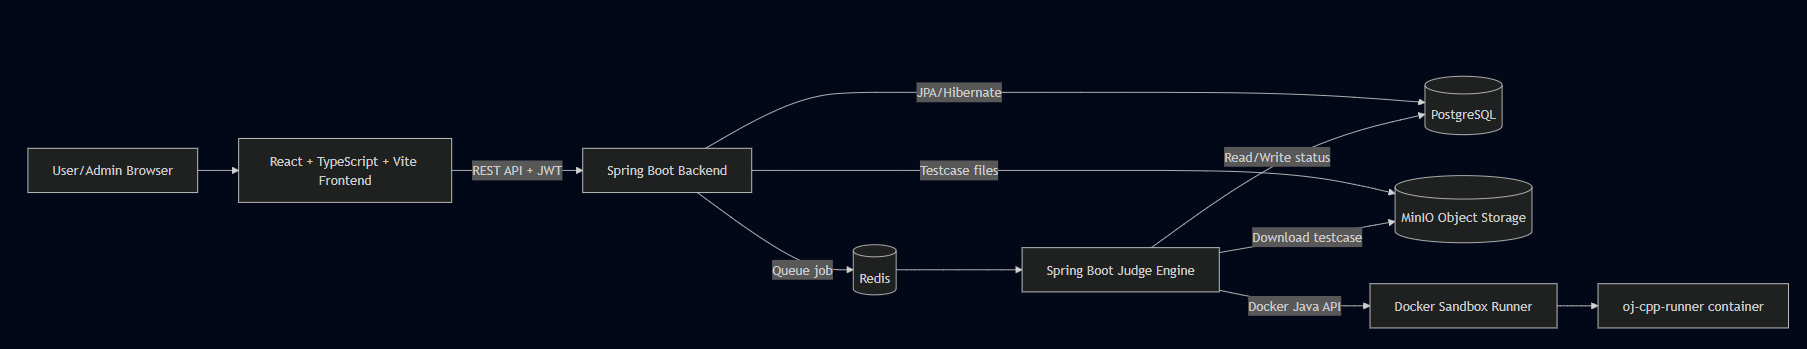
\includegraphics[
        width=\linewidth,
        height=0.45\textheight,
        keepaspectratio
    ]{pic/kientructongthe.png}
    \caption{Kiến trúc tổng thể hệ thống ByeBug}
\end{figure}

\subsection{3. Thành phần chính}

\begin{longtable}[]{
  |>{\raggedright\arraybackslash}p{(\linewidth - 8\tabcolsep) * \real{0.3333}}
  |>{\raggedright\arraybackslash}p{(\linewidth - 8\tabcolsep) * \real{0.3333}}
  |>{\raggedright\arraybackslash}p{(\linewidth - 8\tabcolsep) * \real{0.3333}}|}
\hline\rowcolor{tableHeader}
\begin{minipage}[b]{\linewidth}\raggedright
Thành phần
\end{minipage} & \begin{minipage}[b]{\linewidth}\raggedright
Công nghệ
\end{minipage} & \begin{minipage}[b]{\linewidth}\raggedright
Vai trò
\end{minipage} \\
\hline
\endhead
\hline
\endlastfoot
Frontend & React, TypeScript, Vite, Axios, Monaco Editor & Giao diện người dùng, trang bài tập, trình soạn code, hồ sơ, thống kê, admin dashboard. \\
\hline
Backend API & Java Spring Boot, Spring Security, JWT, JPA/Hibernate & Xử lý nghiệp vụ chính, xác thực, quản lý bài tập, người dùng, submission, notification. \\
\hline
Database & PostgreSQL & Lưu trữ dữ liệu quan hệ: user, admin, problem, testcase, submission, testcase result, notification. \\
\hline
Redis & Redis 7 & Đóng vai trò Message Broker (Hàng đợi gửi job chấm bài) kết nối bất đồng bộ giữa backend và judge engine. \\
\hline
MinIO & Object Storage (S3 Compatible) & Lưu trữ tệp tin testcase input/output và file nguồn nộp bài nhằm giảm tải dung lượng cho DB. \\
\hline
Judge Engine & Java Spring Boot Worker & Lấy job từ Redis, điều phối tài nguyên chạy code trong Docker, cập nhật trạng thái chấm bài (Verdict). \\
\hline
Sandbox & Docker runner image & Biên dịch và thực thi chương trình của người dùng trong môi trường cô lập, an toàn tuyệt đối. \\
\hline
\end{longtable}

\subsection{4. Luồng tương tác chính}

\subsubsection{4.1. Luồng đăng ký/đăng nhập}

\begin{figure}[H]
    \centering
    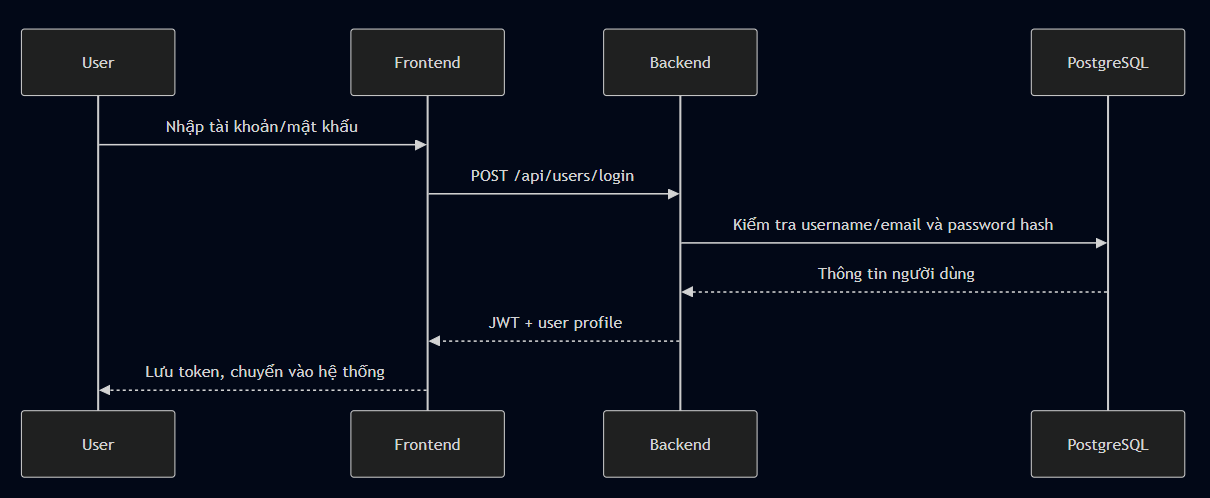
\includegraphics[
        width=\linewidth,
        height=0.45\textheight,
        keepaspectratio
    ]{pic/luongdky_dnhap.png}
    \caption{Luồng đăng ký / đăng nhập}
\end{figure}

\subsubsection{4.2. Luồng xem và tìm kiếm bài tập}

\begin{figure}[H]
    \centering
    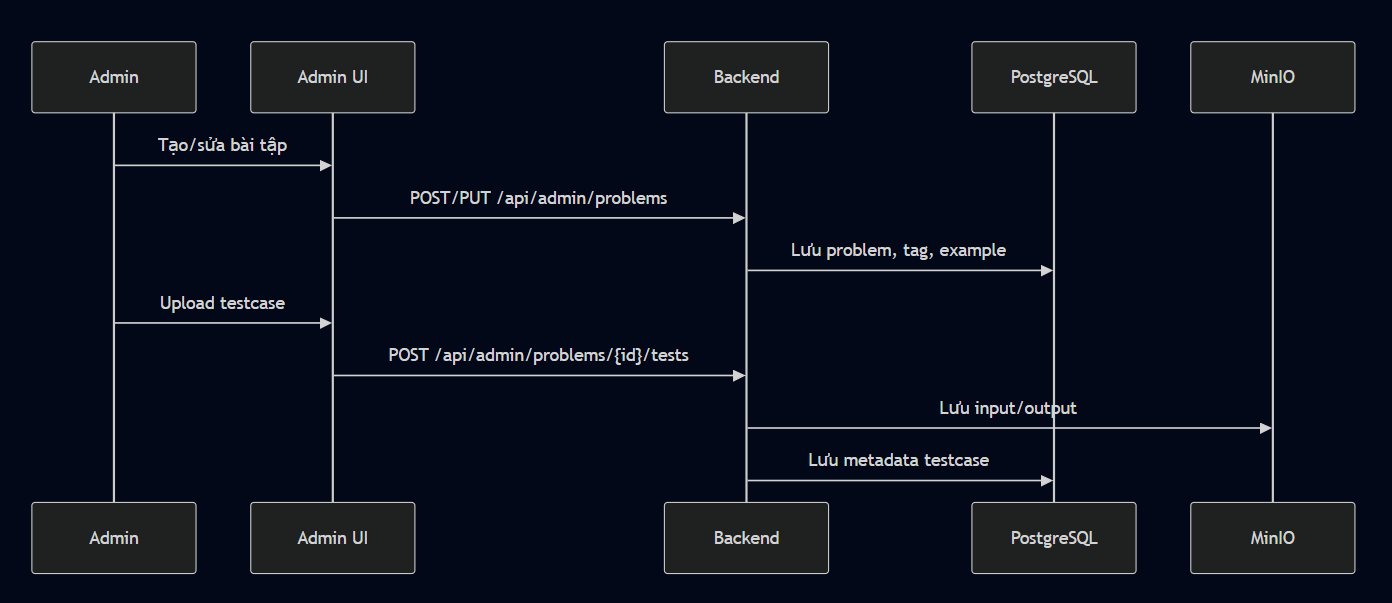
\includegraphics[
        width=\linewidth,
        height=0.45\textheight,
        keepaspectratio
    ]{pic/luong_baitap.png}
    \caption{Luồng xem và tìm kiến bài tập}
    \end{figure}
    


\subsubsection{4.3. Luồng nộp bài và chấm tự động}

\begin{quote}
\textbf{Cơ chế đồng bộ hóa:} Hệ thống sử dụng giải pháp Short-Polling từ Frontend với tần suất \(t = 2s\)/lần sau khi nhận được \texttt{submissionId} từ API Server. Lựa chọn này tối ưu hơn giải pháp kết nối duy trì liên tục (WebSocket) trong môi trường đồ án, giảm thiểu tải kết nối trên API Gateway mà vẫn đảm bảo độ trễ trải nghiệm người dùng (UX Latency) dưới 2000ms.
\end{quote}
\begin{figure}[H]
    \centering
    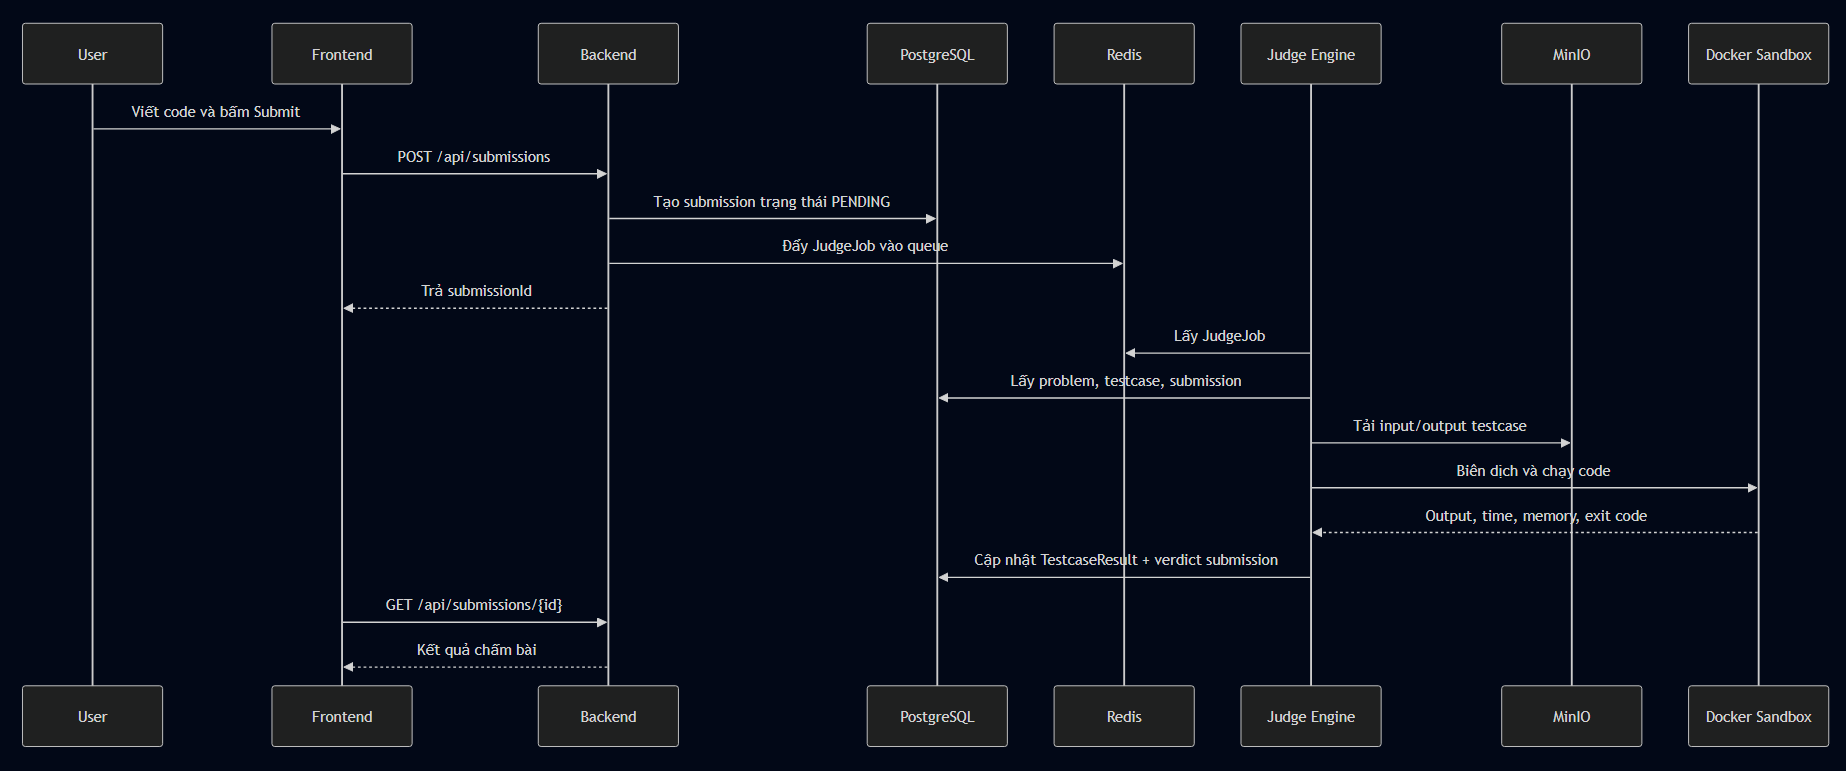
\includegraphics[
        width=\linewidth,
        height=0.45\textheight,
        keepaspectratio
    ]{pic/luong_nopbai.png}
    \caption{Luồng submit}
\end{figure}

\subsubsection{4.4. Luồng quản trị bài tập}
\begin{figure}[H]
    \centering
    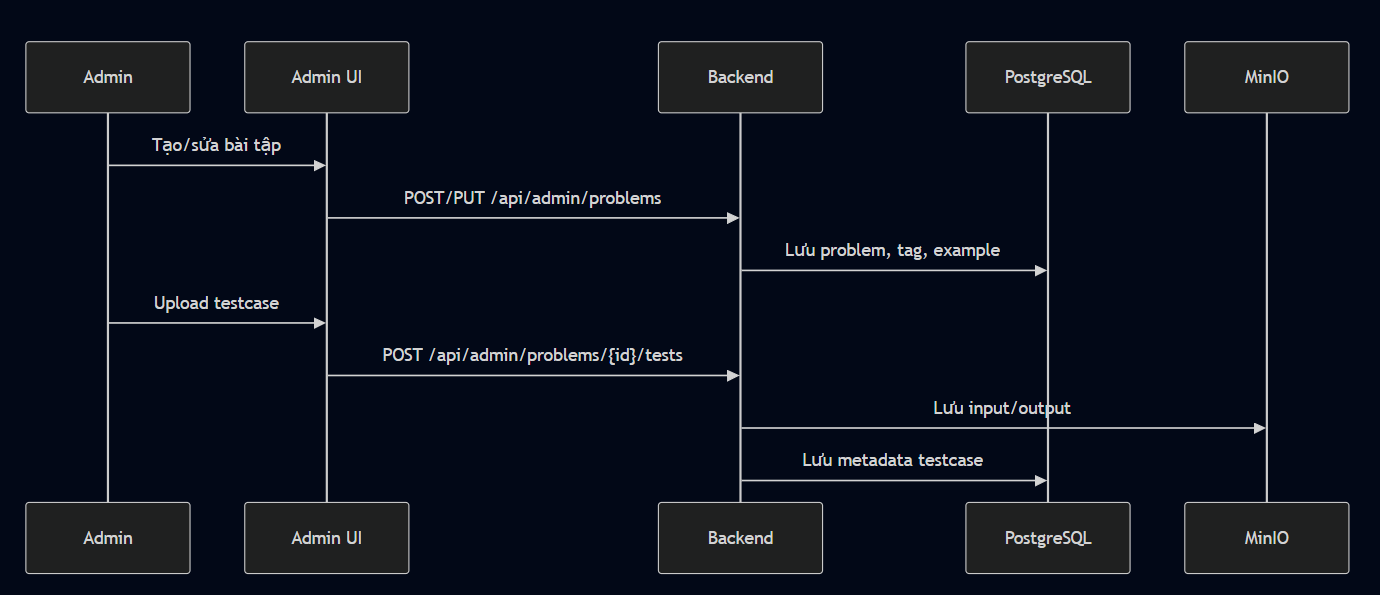
\includegraphics[
        width=\linewidth,
        height=0.45\textheight,
        keepaspectratio
    ]{pic/luong_quantri_baitap.png}
    \caption{Luồng đi quản trị bài tập}
\end{figure}


\subsection{5. Phân quyền và bảo mật cơ bản}

\begin{itemize}
\tightlist
\item
  Người dùng thông thường chỉ được quyền tiếp cận các API public/user (đăng ký, đăng nhập, xem bài public, nộp bài, xem thống kê cá nhân và bảng xếp hạng).
\item
  Admin sử dụng nhóm API riêng biệt cấu hình tiền tố \texttt{/api/admin/} để thực hiện quản lý bài tập, người dùng, cấu hình thông báo và giám sát hệ thống.
\item
  Backend sử dụng cấu hình Spring Security kết hợp với JWT (JSON Web Token). Frontend có trách nhiệm đính kèm token trong mỗi request tại Header dưới dạng \texttt{Authorization:\ Bearer\ \textless{}token\textgreater{}}.
\item
  Toàn bộ mật khẩu của tài khoản đều được băm bằng thuật toán mã hóa một chiều (Password Hashing) trước khi lưu trữ xuống Database, tuyệt đối không lưu chuỗi văn bản thuần (Plaintext).
\end{itemize}

\subsection{6. Chiến lược mở rộng hệ thống (Scalability Strategy)}

\subsubsection{6.1. Mở rộng tầng API Backend}

Backend API có thể mở rộng độc lập theo chiều ngang (Horizontal Scaling) bằng cách triển khai đồng thời nhiều Instance Spring Boot đứng phía sau một bộ cân bằng tải (Load Balancer như Nginx hoặc AWS ALB). Do cơ chế xác thực trạng thái người dùng được đóng gói hoàn toàn trong JWT (Stateless Backend), các Node Backend không cần thực hiện đồng bộ hóa bộ nhớ Session vật lý.
\begin{figure}[H]
    \centering
    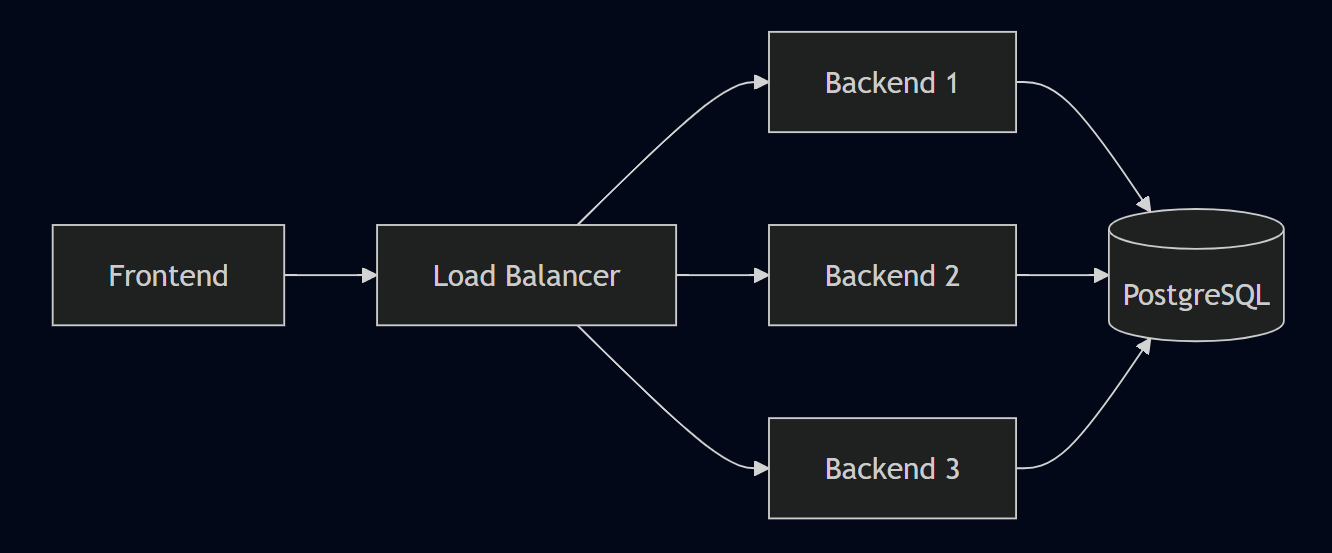
\includegraphics[
        width=\linewidth,
        height=0.45\textheight,
        keepaspectratio
    ]{pic/morong_API_backend.png}
    \caption{Chiến lược mở rộng API Backend}
\end{figure}

\subsubsection{6.2. Mở rộng tầng Judge Engine (Worker Scale)}

Judge Engine được thiết kế tách biệt theo dạng Worker để phục vụ mục đích co giãn linh hoạt. Khi tần suất nộp bài tăng cao đột biến (ví dụ trong các kỳ thi), hệ thống có thể tăng số lượng các Judge Worker cùng lắng nghe và tiêu thụ chung một Redis Queue. Mỗi Worker sẽ tự động kéo một tác vụ (Job) riêng biệt, thực thi chấm và cập nhật trực tiếp kết quả về Database mà không gây tắc nghẽn luồng xử lý của API chính.

\begin{figure}[H]
    \centering
    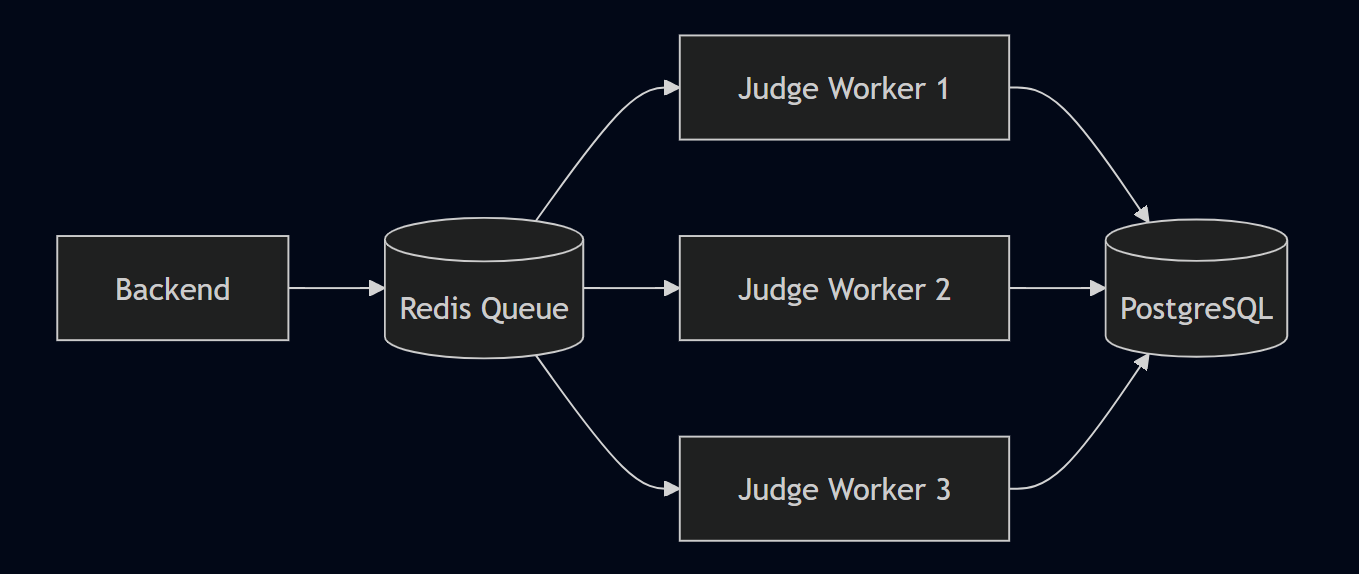
\includegraphics[
        width=\linewidth,
        height=0.45\textheight,
        keepaspectratio
    ]{pic/morong_judgeengine.png}
    \caption{Chiến lược mở rộng Judge Engine - Worker Scale}
\end{figure}
\subsubsection{6.3. Mở rộng hạ tầng lưu trữ}

Tệp tin Testcase dữ liệu đầu vào/đầu ra và mã nguồn giải bài tập được lưu trữ tách biệt hoàn toàn tại Object Storage (MinIO) thay vì lưu trữ dạng nhị phân BLOB trong Database giúp kích thước cơ sở dữ liệu luôn gọn nhẹ, dễ dàng thực hiện sao lưu (Backup) dữ liệu định kỳ.

Khi triển khai trên môi trường Production chạy thật, hệ thống có thể chuyển đổi cấu hình sang các dịch vụ đám mây tương thích như AWS S3 hay Google Cloud Storage mà không cần thay đổi cấu trúc mã nguồn.

\subsubsection{6.4. Cơ chế dọn dẹp và cô lập tài nguyên cục bộ}

Để đảm bảo các Instance Worker khi mở rộng không làm cạn kiệt tài nguyên phần cứng của Host Node:

\begin{itemize}
\tightlist
\item
  \textbf{Container Lifecycle:} Mỗi Docker Sandbox Container chỉ phục vụ biên dịch hoặc thực thi duy nhất cho một tác vụ nộp bài, sau khi hoàn thành sẽ lập tức bị xóa bỏ hoàn toàn (\texttt{docker\ rm\ -f}) để giải phóng tài nguyên bộ nhớ RAM và CPU.
\item
  \textbf{Local Cache Expiry:} Toàn bộ file dữ liệu testcase sau khi tải từ MinIO về bộ nhớ đệm tạm thời (Temporary Directory) của Judge Worker sẽ được thiết lập vòng đời tự động xóa sau khi có Verdict, tránh rò rỉ dung lượng đĩa cứng (Disk Exhaustion).
\end{itemize}

\subsubsection{6.5. Tối ưu hóa truy vấn dữ liệu (Caching \& Indexing)}

\begin{itemize}
\tightlist
\item
  Sử dụng Redis làm tầng Cache đệm lưu trữ dữ liệu cho các chức năng có tần suất truy cập cao nhưng ít biến động liên tục như: Danh sách bài tập tiêu biểu, bảng xếp hạng tổng (Leaderboard).
\item
  Thiết lập phân trang (Pagination) bắt buộc cho toàn bộ các API trả về danh sách lớn (problems, submissions, notifications).
\item
  Khởi tạo chỉ mục (Database Indexing) cho các trường dữ liệu thường xuyên nằm trong điều kiện lọc hoặc sắp xếp: \texttt{username}, \texttt{email}, \texttt{difficulty}, \texttt{is\_public}, \texttt{submitted\_at}, \texttt{total\_score}, \texttt{created\_at}.
\end{itemize}

\subsection{7. Thiết kế an toàn môi trường Sandbox (Security Hardening)}

Để bảo vệ máy chủ Host khỏi các cuộc tấn công mã độc hoặc các đoạn code phá hoại hệ thống do người dùng vô tình hoặc cố ý nộp lên, Docker Sandbox Runner được thiết lập cấu hình nghiêm ngặt:

\begin{itemize}
\tightlist
\item
  \textbf{Hạn chế đặc quyền (Non-root User):} Tiến trình thực thi mã nguồn của người dùng bên trong Container được chỉ định chạy dưới quyền của User không có đặc quyền hệ thống (\texttt{nobody}), loại bỏ nguy cơ chiếm quyền điều khiển tài nguyên vật lý.
\item
  \textbf{Cô lập mạng hoàn toàn (Network Isolation):} Khởi chạy Sandbox Container với tham số mạng \texttt{-\/-network\ none}. Đoạn mã của người dùng hoàn toàn bị cắt đứt kết nối Internet, không thể gửi yêu cầu HTTP ra ngoài, không thể tải mã độc hoặc thực hiện các hành vi tấn công DDoS ngược lại mạng nội bộ.
\item
  \textbf{Giới hạn tiến trình (Fork Bomb Protection):} Cấu hình chặt chẽ giới hạn số lượng tiến trình con được phép sinh ra trong container thông qua cờ \texttt{-\/-pids-limit\ 64}, ngăn chặn triệt để các cuộc tấn công từ chối dịch vụ dạng Fork Bomb làm treo hệ thống máy chủ.
\end{itemize}

\subsection{8. Rủi ro kỹ thuật và hướng xử lý}

\begin{longtable}[]{
  |>{\raggedright\arraybackslash}p{(\linewidth - 8\tabcolsep) * \real{0.3333}}
  |>{\raggedright\arraybackslash}p{(\linewidth - 8\tabcolsep) * \real{0.3333}}
  |>{\raggedright\arraybackslash}p{(\linewidth - 8\tabcolsep) * \real{0.3333}}|}
\hline\rowcolor{tableHeader}
\begin{minipage}[b]{\linewidth}\raggedright
Rủi ro
\end{minipage} & \begin{minipage}[b]{\linewidth}\raggedright
Ảnh hưởng
\end{minipage} & \begin{minipage}[b]{\linewidth}\raggedright
Hướng xử lý
\end{minipage} \\
\hline
\endhead
\hline
\endlastfoot
Mã nguồn người dùng chạy vô hạn & Gây nghẽn luồng xử lý của Judge Worker, treo tài nguyên hệ thống. & Cấu hình giới hạn thời gian chạy tối đa (Time Limit), áp dụng cơ chế tự động ngắt tiến trình (Timeout Process) hoặc cưỡng chế tắt container từ phía Worker. \\
\hline
Mã nguồn tiêu tốn quá nhiều RAM & Gây sập hoặc làm chậm Host Machine (Lỗi Out Of Memory). & Giới hạn dung lượng bộ nhớ tối đa được phép phân bổ cho Container thông qua cấu hình giới hạn RAM của Docker (\texttt{-\/-memory}). \\
\hline
Hàng đợi nộp bài tăng nhanh & Thời gian chờ đợi kết quả chấm bài của người dùng bị kéo dài (UX kém). & Thiết lập hệ thống giám sát độ dài hàng đợi (Queue Length Monitoring), kích hoạt cơ chế tự động nhân bản thêm Judge Worker (Auto-scaling) khi hàng đợi vượt ngưỡng cảnh báo. \\
\hline
Database rơi vào trạng thái quá tải & Độ trễ của toàn bộ hệ thống API tăng mạnh, có thể gây sập kết nối DB. & Tối ưu hóa Index, áp dụng bộ đệm Cache Redis, phân trang nghiêm ngặt, thực hiện tách biệt cơ sở dữ liệu đọc/ghi (Read/Write Replicas) nếu cần thiết. \\
\hline
Rò rỉ dữ liệu Testcase & Làm mất tính công bằng và minh bạch của các cuộc thi trực tuyến. & Cấu hình MinIO Bucket ở chế độ riêng tư (Private Bucket), chỉ cho phép Backend API và Judge Engine truy cập thông qua tài khoản định danh nội bộ có thời hạn Presigned URL ngắn. \\
\hline
\end{longtable}

\newpage

\section{CHƯƠNG 2. Thiết kế cơ sở dữ liệu ByeBug}

\subsection{1. Tổng quan hệ thống dữ liệu}

Hệ thống ByeBug lựa chọn cơ sở dữ liệu quan hệ PostgreSQL làm nền tảng lưu trữ chính, tương tác thông qua tầng Spring Data JPA/Hibernate tại Backend Server. Dữ liệu tệp tin có dung lượng lớn và tần suất thay đổi thấp (như các tệp tin dữ liệu đầu vào \texttt{.in} và đầu ra \texttt{.out} của các bộ Testcase) được lưu trữ độc lập ngoài cơ sở dữ liệu thông qua hệ thống MinIO Object Storage; cơ sở dữ liệu PostgreSQL chỉ chịu trách nhiệm quản lý thông tin định danh (Metadata) và đường dẫn tệp tin (Object Key).

\subsection{2. Hệ thống các bảng chi tiết (Tables Metadata)}

\subsubsection{\texorpdfstring{2.1. Bảng: \texttt{users} --- Quản lý tài khoản học viên}{2.1. Bảng: users --- Quản lý tài khoản học viên}}

\begin{longtable}[]{
  |>{\raggedright\arraybackslash}p{(\linewidth - 10\tabcolsep) * \real{0.2500}}
  |>{\raggedright\arraybackslash}p{(\linewidth - 10\tabcolsep) * \real{0.2500}}
  |>{\raggedright\arraybackslash}p{(\linewidth - 10\tabcolsep) * \real{0.2500}}
  |>{\raggedright\arraybackslash}p{(\linewidth - 10\tabcolsep) * \real{0.2500}}|}
\hline\rowcolor{tableHeader}
\begin{minipage}[b]{\linewidth}\raggedright
Tên trường
\end{minipage} & \begin{minipage}[b]{\linewidth}\raggedright
Kiểu dữ liệu
\end{minipage} & \begin{minipage}[b]{\linewidth}\raggedright
Ràng buộc
\end{minipage} & \begin{minipage}[b]{\linewidth}\raggedright
Mô tả
\end{minipage} \\
\hline
\endhead
\hline
\endlastfoot
\texttt{user\_id} & \texttt{BIGSERIAL} & PRIMARY KEY & Khóa chính tự tăng của người dùng. \\
\hline
\texttt{username} & \texttt{VARCHAR(50)} & UNIQUE, NOT NULL & Tên đăng nhập hệ thống. \\
\hline
\texttt{full\_name} & \texttt{VARCHAR(100)} & NOT NULL & Họ và tên hiển thị trên giao diện. \\
\hline
\texttt{email} & \texttt{VARCHAR(100)} & UNIQUE, NOT NULL & Địa chỉ email người dùng. \\
\hline
\texttt{password\_hash} & \texttt{VARCHAR(255)} & NOT NULL & Mật khẩu đã mã hóa một chiều qua BCrypt. \\
\hline
\texttt{avatar\_url} & \texttt{TEXT} & NULL & Đường dẫn ảnh đại diện (Lưu trên Object Storage). \\
\hline
\texttt{gender} & \texttt{VARCHAR(10)} & NULL & Giới tính của người dùng. \\
\hline
\texttt{role} & \texttt{VARCHAR(20)} & DEFAULT `USER' & Vai trò hệ thống, mặc định là \texttt{USER}. \\
\hline
\texttt{total\_score} & \texttt{INTEGER} & DEFAULT 0 & Tổng điểm tích lũy dùng để xếp hạng Leaderboard. \\
\hline
\texttt{is\_active} & \texttt{BOOLEAN} & DEFAULT TRUE & Trạng thái kích hoạt của tài khoản. \\
\hline
\texttt{created\_at} & \texttt{TIMESTAMP} & DEFAULT NOW() & Thời điểm khởi tạo tài khoản. \\
\hline
\texttt{last\_login\_at} & \texttt{TIMESTAMP} & NULL & Thời điểm thực hiện lần đăng nhập gần nhất. \\
\hline
\texttt{deleted\_at} & \texttt{TIMESTAMP} & NULL & Đánh dấu thời gian xóa tài khoản (Soft Delete). \\
\hline
\end{longtable}

\subsubsection{\texorpdfstring{2.2. Bảng: \texttt{admins} --- Quản lý tài khoản quản trị hệ thống}{2.2. Bảng: admins --- Quản lý tài khoản quản trị hệ thống}}

\begin{longtable}[]{
  |>{\raggedright\arraybackslash}p{(\linewidth - 10\tabcolsep) * \real{0.2500}}
  |>{\raggedright\arraybackslash}p{(\linewidth - 10\tabcolsep) * \real{0.2500}}
  |>{\raggedright\arraybackslash}p{(\linewidth - 10\tabcolsep) * \real{0.2500}}
  |>{\raggedright\arraybackslash}p{(\linewidth - 10\tabcolsep) * \real{0.2500}}|}
\hline\rowcolor{tableHeader}
\begin{minipage}[b]{\linewidth}\raggedright
Tên trường
\end{minipage} & \begin{minipage}[b]{\linewidth}\raggedright
Kiểu dữ liệu
\end{minipage} & \begin{minipage}[b]{\linewidth}\raggedright
Ràng buộc
\end{minipage} & \begin{minipage}[b]{\linewidth}\raggedright
Mô tả
\end{minipage} \\
\hline
\endhead
\hline
\endlastfoot
\texttt{admin\_id} & \texttt{BIGSERIAL} & PRIMARY KEY & Khóa chính hệ thống admin. \\
\hline
\texttt{username} & \texttt{VARCHAR(50)} & UNIQUE, NOT NULL & Tên đăng nhập của admin. \\
\hline
\texttt{full\_name} & \texttt{VARCHAR(100)} & NOT NULL & Họ tên hiển thị của admin. \\
\hline
\texttt{email} & \texttt{VARCHAR(100)} & UNIQUE, NOT NULL & Email liên hệ của admin. \\
\hline
\texttt{password\_hash} & \texttt{VARCHAR(255)} & NOT NULL & Mật khẩu đã mã hóa của admin. \\
\hline
\texttt{avatar\_url} & \texttt{TEXT} & NULL & Đường dẫn ảnh đại diện của quản trị viên. \\
\hline
\texttt{is\_active} & \texttt{BOOLEAN} & DEFAULT TRUE & Trạng thái hoạt động của tài khoản admin. \\
\hline
\texttt{created\_at} & \texttt{TIMESTAMP} & DEFAULT NOW() & Thời điểm khởi tạo tài khoản quản trị. \\
\hline
\end{longtable}

\subsubsection{\texorpdfstring{2.3. Bảng: \texttt{problems} --- Thông tin bài tập lập trình}{2.3. Bảng: problems --- Thông tin bài tập lập trình}}

\begin{longtable}[]{
  |>{\raggedright\arraybackslash}p{(\linewidth - 10\tabcolsep) * \real{0.2500}}
  |>{\raggedright\arraybackslash}p{(\linewidth - 10\tabcolsep) * \real{0.2500}}
  |>{\raggedright\arraybackslash}p{(\linewidth - 10\tabcolsep) * \real{0.2500}}
  |>{\raggedright\arraybackslash}p{(\linewidth - 10\tabcolsep) * \real{0.2500}}|}
\hline\rowcolor{tableHeader}
\begin{minipage}[b]{\linewidth}\raggedright
Tên trường
\end{minipage} & \begin{minipage}[b]{\linewidth}\raggedright
Kiểu dữ liệu
\end{minipage} & \begin{minipage}[b]{\linewidth}\raggedright
Ràng buộc
\end{minipage} & \begin{minipage}[b]{\linewidth}\raggedright
Mô tả
\end{minipage} \\
\hline
\endhead
\hline
\endlastfoot
\texttt{problem\_id} & \texttt{BIGSERIAL} & PRIMARY KEY & Khóa chính bài toán. \\
\hline
\texttt{title} & \texttt{VARCHAR(255)} & NOT NULL & Tiêu đề của bài tập. \\
\hline
\texttt{description} & \texttt{TEXT} & NOT NULL & Nội dung chi tiết đề bài (Định dạng Markdown). \\
\hline
\texttt{constraints} & \texttt{TEXT} & NULL & Các ràng buộc đặc biệt của bài toán. \\
\hline
\texttt{difficulty} & \texttt{VARCHAR(20)} & NOT NULL & Độ khó bài toán: \texttt{EASY}, \texttt{MEDIUM}, \texttt{HARD}. \\
\hline
\texttt{time\_limit\_ms} & \texttt{INTEGER} & NOT NULL & Giới hạn thời gian chạy tối đa (mili-giây). \\
\hline
\texttt{memory\_limit\_kb} & \texttt{INTEGER} & NOT NULL & Giới hạn bộ nhớ RAM tối đa cấp phát (KB). \\
\hline
\texttt{allow\_file\_submit} & \texttt{BOOLEAN} & DEFAULT FALSE & Cho phép người dùng nộp bài bằng cách tải tệp tin. \\
\hline
\texttt{is\_public} & \texttt{BOOLEAN} & DEFAULT FALSE & Trạng thái hiển thị công khai trên hệ thống. \\
\hline
\texttt{creator\_id} & \texttt{BIGINT} & FOREIGN KEY & Liên kết đến \texttt{admins.admin\_id} (Người biên soạn). \\
\hline
\texttt{created\_at} & \texttt{TIMESTAMP} & DEFAULT NOW() & Thời điểm khởi tạo bài toán. \\
\hline
\end{longtable}

\subsubsection{\texorpdfstring{2.4. Bảng: \texttt{tags} --- Danh mục phân loại thuật toán}{2.4. Bảng: tags --- Danh mục phân loại thuật toán}}

\begin{longtable}[]{
  |>{\raggedright\arraybackslash}p{(\linewidth - 10\tabcolsep) * \real{0.2500}}
  |>{\raggedright\arraybackslash}p{(\linewidth - 10\tabcolsep) * \real{0.2500}}
  |>{\raggedright\arraybackslash}p{(\linewidth - 10\tabcolsep) * \real{0.2500}}
  |>{\raggedright\arraybackslash}p{(\linewidth - 10\tabcolsep) * \real{0.2500}}|}
\hline\rowcolor{tableHeader}
\begin{minipage}[b]{\linewidth}\raggedright
Tên trường
\end{minipage} & \begin{minipage}[b]{\linewidth}\raggedright
Kiểu dữ liệu
\end{minipage} & \begin{minipage}[b]{\linewidth}\raggedright
Ràng buộc
\end{minipage} & \begin{minipage}[b]{\linewidth}\raggedright
Mô tả
\end{minipage} \\
\hline
\endhead
\hline
\endlastfoot
\texttt{tag\_id} & \texttt{SERIAL} & PRIMARY KEY & Khóa chính danh mục tag. \\
\hline
\texttt{tag\_name} & \texttt{VARCHAR(50)} & UNIQUE, NOT NULL & Tên thẻ phân loại (Ví dụ: Array, Math, DP, Graph). \\
\hline
\end{longtable}

\subsubsection{\texorpdfstring{2.5. Bảng: \texttt{problem\_tags} --- Quan hệ Nhiều-Nhiều giữa Problem và Tag}{2.5. Bảng: problem\_tags --- Quan hệ Nhiều-Nhiều giữa Problem và Tag}}

\begin{longtable}[]{
  |>{\raggedright\arraybackslash}p{(\linewidth - 10\tabcolsep) * \real{0.2500}}
  |>{\raggedright\arraybackslash}p{(\linewidth - 10\tabcolsep) * \real{0.2500}}
  |>{\raggedright\arraybackslash}p{(\linewidth - 10\tabcolsep) * \real{0.2500}}
  |>{\raggedright\arraybackslash}p{(\linewidth - 10\tabcolsep) * \real{0.2500}}|}
\hline\rowcolor{tableHeader}
\begin{minipage}[b]{\linewidth}\raggedright
Tên trường
\end{minipage} & \begin{minipage}[b]{\linewidth}\raggedright
Kiểu dữ liệu
\end{minipage} & \begin{minipage}[b]{\linewidth}\raggedright
Ràng buộc
\end{minipage} & \begin{minipage}[b]{\linewidth}\raggedright
Mô tả
\end{minipage} \\
\hline
\endhead
\hline
\endlastfoot
\texttt{problem\_id} & \texttt{BIGINT} & FOREIGN KEY, PK & Liên kết đến mã bài toán \texttt{problems.problem\_id}. \\
\hline
\texttt{tag\_id} & \texttt{INTEGER} & FOREIGN KEY, PK & Liên kết đến mã danh mục \texttt{tags.tag\_id}. \\
\hline
\end{longtable}

\subsubsection{\texorpdfstring{2.6. Bảng: \texttt{problem\_examples} --- Dữ liệu ví dụ mẫu hiển thị tại đề bài}{2.6. Bảng: problem\_examples --- Dữ liệu ví dụ mẫu hiển thị tại đề bài}}

\begin{longtable}[]{
  |>{\raggedright\arraybackslash}p{(\linewidth - 10\tabcolsep) * \real{0.2500}}
  |>{\raggedright\arraybackslash}p{(\linewidth - 10\tabcolsep) * \real{0.2500}}
  |>{\raggedright\arraybackslash}p{(\linewidth - 10\tabcolsep) * \real{0.2500}}
  |>{\raggedright\arraybackslash}p{(\linewidth - 10\tabcolsep) * \real{0.2500}}|}
\hline\rowcolor{tableHeader}
\begin{minipage}[b]{\linewidth}\raggedright
Tên trường
\end{minipage} & \begin{minipage}[b]{\linewidth}\raggedright
Kiểu dữ liệu
\end{minipage} & \begin{minipage}[b]{\linewidth}\raggedright
Ràng buộc
\end{minipage} & \begin{minipage}[b]{\linewidth}\raggedright
Mô tả
\end{minipage} \\
\hline
\endhead
\hline
\endlastfoot
\texttt{example\_id} & \texttt{BIGSERIAL} & PRIMARY KEY & Khóa chính dữ liệu ví dụ. \\
\hline
\texttt{problem\_id} & \texttt{BIGINT} & FOREIGN KEY & Liên kết đến bài toán chứa ví dụ mẫu này. \\
\hline
\texttt{input} & \texttt{TEXT} & NOT NULL & Dữ liệu đầu vào mẫu hiển thị cho học viên. \\
\hline
\texttt{output} & \texttt{TEXT} & NOT NULL & Dữ liệu đầu ra mẫu kỳ vọng tương ứng. \\
\hline
\texttt{explanation} & \texttt{TEXT} & NULL & Đoạn văn bản giải thích luồng thuật toán của ví dụ. \\
\hline
\texttt{display\_order} & \texttt{INTEGER} & DEFAULT 1 & Thứ tự sắp xếp hiển thị trên giao diện đề bài. \\
\hline
\end{longtable}

\subsubsection{\texorpdfstring{2.7. Bảng: \texttt{testcases} --- Hệ thống dữ liệu kiểm thử ẩn dùng để chấm bài}{2.7. Bảng: testcases --- Hệ thống dữ liệu kiểm thử ẩn dùng để chấm bài}}

\begin{longtable}[]{
  |>{\raggedright\arraybackslash}p{(\linewidth - 10\tabcolsep) * \real{0.2500}}
  |>{\raggedright\arraybackslash}p{(\linewidth - 10\tabcolsep) * \real{0.2500}}
  |>{\raggedright\arraybackslash}p{(\linewidth - 10\tabcolsep) * \real{0.2500}}
  |>{\raggedright\arraybackslash}p{(\linewidth - 10\tabcolsep) * \real{0.2500}}|}
\hline\rowcolor{tableHeader}
\begin{minipage}[b]{\linewidth}\raggedright
Tên trường
\end{minipage} & \begin{minipage}[b]{\linewidth}\raggedright
Kiểu dữ liệu
\end{minipage} & \begin{minipage}[b]{\linewidth}\raggedright
Ràng buộc
\end{minipage} & \begin{minipage}[b]{\linewidth}\raggedright
Mô tả
\end{minipage} \\
\hline
\endhead
\hline
\endlastfoot
\texttt{testcase\_id} & \texttt{BIGSERIAL} & PRIMARY KEY & Khóa chính của bộ testcase. \\
\hline
\texttt{problem\_id} & \texttt{BIGINT} & FOREIGN KEY & Bài toán sở hữu testcase, kết nối với \texttt{problems}. \\
\hline
\texttt{input\_path} & \texttt{TEXT} & NOT NULL & Mã định danh Object Key lưu tệp tin đầu vào tại MinIO. \\
\hline
\texttt{output\_path} & \texttt{TEXT} & NOT NULL & Mã định danh Object Key lưu tệp tin đầu ra tại MinIO. \\
\hline
\texttt{is\_visible} & \texttt{BOOLEAN} & DEFAULT FALSE & Xác định hệ thống có cho phép hiển thị bộ test này không. \\
\hline
\texttt{display\_order} & \texttt{INTEGER} & DEFAULT 1 & Thứ tự tuần tự khi Judge Worker gọi chạy test. \\
\hline
\texttt{score\_weight} & \texttt{INTEGER} & DEFAULT 10 & Trọng số điểm đạt được khi vượt qua testcase này. \\
\hline
\end{longtable}

\subsubsection{\texorpdfstring{2.8. Bảng: \texttt{submissions} --- Nhật ký các lượt nộp bài làm của học viên}{2.8. Bảng: submissions --- Nhật ký các lượt nộp bài làm của học viên}}

\begin{longtable}[]{
  |>{\raggedright\arraybackslash}p{(\linewidth - 10\tabcolsep) * \real{0.2500}}
  |>{\raggedright\arraybackslash}p{(\linewidth - 10\tabcolsep) * \real{0.2500}}
  |>{\raggedright\arraybackslash}p{(\linewidth - 10\tabcolsep) * \real{0.2500}}
  |>{\raggedright\arraybackslash}p{(\linewidth - 10\tabcolsep) * \real{0.2500}}|}
\hline\rowcolor{tableHeader}
\begin{minipage}[b]{\linewidth}\raggedright
Tên trường
\end{minipage} & \begin{minipage}[b]{\linewidth}\raggedright
Kiểu dữ liệu
\end{minipage} & \begin{minipage}[b]{\linewidth}\raggedright
Ràng buộc
\end{minipage} & \begin{minipage}[b]{\linewidth}\raggedright
Mô tả
\end{minipage} \\
\hline
\endhead
\hline
\endlastfoot
\texttt{submission\_id} & \texttt{BIGSERIAL} & PRIMARY KEY & Khóa chính của lượt nộp bài. \\
\hline
\texttt{problem\_id} & \texttt{BIGINT} & FOREIGN KEY & Bài toán được giải, kết nối với \texttt{problems}. \\
\hline
\texttt{user\_id} & \texttt{BIGINT} & FOREIGN KEY & Người thực hiện nộp bài, kết nối với \texttt{users}. \\
\hline
\texttt{language} & \texttt{VARCHAR(20)} & NOT NULL & Ngôn ngữ sử dụng lập trình (\texttt{cpp}, \texttt{java}, \texttt{python}). \\
\hline
\texttt{source\_code} & \texttt{TEXT} & NULL & Mã nguồn giải bài (nếu gõ trực tiếp trên Editor). \\
\hline
\texttt{file\_url} & \texttt{TEXT} & NULL & Đường dẫn file mã nguồn nếu chọn phương thức nộp file. \\
\hline
\texttt{verdict} & \texttt{VARCHAR(30)} & DEFAULT `PENDING' & Trạng thái chấm: \texttt{PENDING}, \texttt{AC}, \texttt{WA}, \texttt{TLE}, \texttt{MLE}, \texttt{CE}\ldots{} \\
\hline
\texttt{compile\_error} & \texttt{TEXT} & NULL & Nội dung chi tiết lỗi log trả về từ trình biên dịch. \\
\hline
\texttt{judge\_message} & \texttt{TEXT} & NULL & Thông báo bổ sung từ hệ thống Judge Engine. \\
\hline
\texttt{score} & \texttt{INTEGER} & DEFAULT 0 & Tổng điểm số thu về của lượt nộp bài này. \\
\hline
\texttt{total\_time\_ms} & \texttt{INTEGER} & DEFAULT 0 & Thời gian thực thi lâu nhất trong các testcase (ms). \\
\hline
\texttt{max\_memory\_kb} & \texttt{INTEGER} & DEFAULT 0 & Dung lượng bộ nhớ lớn nhất ghi nhận được (KB). \\
\hline
\texttt{submitted\_at} & \texttt{TIMESTAMP} & DEFAULT NOW() & Thời điểm hệ thống ghi nhận lượt nộp bài. \\
\hline
\end{longtable}

\subsubsection{\texorpdfstring{2.9. Bảng: \texttt{testcase\_results} --- Chi tiết kết quả thực thi trên từng bộ testcase}{2.9. Bảng: testcase\_results --- Chi tiết kết quả thực thi trên từng bộ testcase}}

\begin{longtable}[]{
  |>{\raggedright\arraybackslash}p{(\linewidth - 10\tabcolsep) * \real{0.2500}}
  |>{\raggedright\arraybackslash}p{(\linewidth - 10\tabcolsep) * \real{0.2500}}
  |>{\raggedright\arraybackslash}p{(\linewidth - 10\tabcolsep) * \real{0.2500}}
  |>{\raggedright\arraybackslash}p{(\linewidth - 10\tabcolsep) * \real{0.2500}}|}
\hline\rowcolor{tableHeader}
\begin{minipage}[b]{\linewidth}\raggedright
Tên trường
\end{minipage} & \begin{minipage}[b]{\linewidth}\raggedright
Kiểu dữ liệu
\end{minipage} & \begin{minipage}[b]{\linewidth}\raggedright
Ràng buộc
\end{minipage} & \begin{minipage}[b]{\linewidth}\raggedright
Mô tả
\end{minipage} \\
\hline
\endhead
\hline
\endlastfoot
\texttt{id} & \texttt{BIGSERIAL} & PRIMARY KEY & Khóa chính kết quả kiểm thử. \\
\hline
\texttt{submission\_id} & \texttt{BIGINT} & FOREIGN KEY & Thuộc lượt nộp bài nào, kết nối với \texttt{submissions}. \\
\hline
\texttt{testcase\_id} & \texttt{BIGINT} & FOREIGN KEY & Liên kết đối chiếu sang danh mục bộ test \texttt{testcases}. \\
\hline
\texttt{verdict} & \texttt{VARCHAR(30)} & NOT NULL & Kết quả đánh giá trên bộ test này (\texttt{AC}, \texttt{WA}, \texttt{TLE}\ldots). \\
\hline
\texttt{user\_output} & \texttt{TEXT} & NULL & Dữ liệu đầu ra do mã nguồn của người dùng sinh ra. \\
\hline
\texttt{time\_ms} & \texttt{INTEGER} & NOT NULL & Thời gian thực thi chi tiết trên cấu hình testcase (ms). \\
\hline
\texttt{memory\_kb} & \texttt{INTEGER} & NOT NULL & Bộ nhớ tiêu tốn chi tiết trên cấu hình testcase (KB). \\
\hline
\end{longtable}

\subsubsection{\texorpdfstring{2.10. Bảng: \texttt{notification\_broadcasts} --- Kho lưu trữ nội dung thông báo gốc từ ban quản trị}{2.10. Bảng: notification\_broadcasts --- Kho lưu trữ nội dung thông báo gốc từ ban quản trị}}

\begin{longtable}[]{
  |>{\raggedright\arraybackslash}p{(\linewidth - 10\tabcolsep) * \real{0.2500}}
  |>{\raggedright\arraybackslash}p{(\linewidth - 10\tabcolsep) * \real{0.2500}}
  |>{\raggedright\arraybackslash}p{(\linewidth - 10\tabcolsep) * \real{0.2500}}
  |>{\raggedright\arraybackslash}p{(\linewidth - 10\tabcolsep) * \real{0.2500}}|}
\hline\rowcolor{tableHeader}
\begin{minipage}[b]{\linewidth}\raggedright
Tên trường
\end{minipage} & \begin{minipage}[b]{\linewidth}\raggedright
Kiểu dữ liệu
\end{minipage} & \begin{minipage}[b]{\linewidth}\raggedright
Ràng buộc
\end{minipage} & \begin{minipage}[b]{\linewidth}\raggedright
Mô tả
\end{minipage} \\
\hline
\endhead
\hline
\endlastfoot
\texttt{broadcast\_id} & \texttt{BIGSERIAL} & PRIMARY KEY & Khóa chính thông báo gốc. \\
\hline
\texttt{title} & \texttt{VARCHAR(255)} & NOT NULL & Tiêu đề hiển thị của thông báo. \\
\hline
\texttt{content} & \texttt{TEXT} & NOT NULL & Nội dung chi tiết của thông báo gửi đi. \\
\hline
\texttt{audience\_type} & \texttt{VARCHAR(30)} & NOT NULL & Phân loại nhóm đối tượng nhận thông báo. \\
\hline
\texttt{priority} & \texttt{VARCHAR(20)} & DEFAULT `NORMAL' & Mức độ khẩn cấp của thông báo (\texttt{LOW}, \texttt{NORMAL}, \texttt{HIGH}). \\
\hline
\texttt{created\_by\_admin\_id} & \texttt{BIGINT} & FOREIGN KEY & Định danh admin tạo thông báo, kết nối với \texttt{admins}. \\
\hline
\texttt{scheduled\_at} & \texttt{TIMESTAMP} & NULL & Thiết lập lịch phát thông báo tự động trong tương lai. \\
\hline
\texttt{created\_at} & \texttt{TIMESTAMP} & DEFAULT NOW() & Thời gian biên soạn nội dung thông báo. \\
\hline
\end{longtable}

\subsubsection{\texorpdfstring{2.11. Bảng: \texttt{notifications} --- Quản lý trạng thái tiếp nhận thông báo của từng học viên}{2.11. Bảng: notifications --- Quản lý trạng thái tiếp nhận thông báo của từng học viên}}

\begin{longtable}[]{
  |>{\raggedright\arraybackslash}p{(\linewidth - 10\tabcolsep) * \real{0.2500}}
  |>{\raggedright\arraybackslash}p{(\linewidth - 10\tabcolsep) * \real{0.2500}}
  |>{\raggedright\arraybackslash}p{(\linewidth - 10\tabcolsep) * \real{0.2500}}
  |>{\raggedright\arraybackslash}p{(\linewidth - 10\tabcolsep) * \real{0.2500}}|}
\hline\rowcolor{tableHeader}
\begin{minipage}[b]{\linewidth}\raggedright
Tên trường
\end{minipage} & \begin{minipage}[b]{\linewidth}\raggedright
Kiểu dữ liệu
\end{minipage} & \begin{minipage}[b]{\linewidth}\raggedright
Ràng buộc
\end{minipage} & \begin{minipage}[b]{\linewidth}\raggedright
Mô tả
\end{minipage} \\
\hline
\endhead
\hline
\endlastfoot
\texttt{notification\_id} & \texttt{BIGSERIAL} & PRIMARY KEY & Khóa chính bản ghi nhận. \\
\hline
\texttt{broadcast\_id} & \texttt{BIGINT} & FOREIGN KEY & Liên kết sang thông báo gốc \texttt{notification\_broadcasts}. \\
\hline
\texttt{user\_id} & \texttt{BIGINT} & FOREIGN KEY & Người nhận thông báo, kết nối với bảng \texttt{users}. \\
\hline
\texttt{is\_read} & \texttt{BOOLEAN} & DEFAULT FALSE & Trạng thái người dùng đã đọc thông báo hay chưa. \\
\hline
\texttt{created\_at} & \texttt{TIMESTAMP} & DEFAULT NOW() & Thời điểm gửi thông báo đến hộp thư người dùng. \\
\hline
\end{longtable}

\subsubsection{\texorpdfstring{2.12. Bảng: \texttt{admin\_notifications} --- Quản lý trạng thái tiếp nhận thông báo nội bộ của Admin}{2.12. Bảng: admin\_notifications --- Quản lý trạng thái tiếp nhận thông báo nội bộ của Admin}}

\begin{longtable}[]{
  |>{\raggedright\arraybackslash}p{(\linewidth - 10\tabcolsep) * \real{0.2500}}
  |>{\raggedright\arraybackslash}p{(\linewidth - 10\tabcolsep) * \real{0.2500}}
  |>{\raggedright\arraybackslash}p{(\linewidth - 10\tabcolsep) * \real{0.2500}}
  |>{\raggedright\arraybackslash}p{(\linewidth - 10\tabcolsep) * \real{0.2500}}|}
\hline\rowcolor{tableHeader}
\begin{minipage}[b]{\linewidth}\raggedright
Tên trường
\end{minipage} & \begin{minipage}[b]{\linewidth}\raggedright
Kiểu dữ liệu
\end{minipage} & \begin{minipage}[b]{\linewidth}\raggedright
Ràng buộc
\end{minipage} & \begin{minipage}[b]{\linewidth}\raggedright
Mô tả
\end{minipage} \\
\hline
\endhead
\hline
\endlastfoot
\texttt{admin\_notification\_id} & \texttt{BIGSERIAL} & PRIMARY KEY & Khóa chính bản ghi nhận. \\
\hline
\texttt{broadcast\_id} & \texttt{BIGINT} & FOREIGN KEY & Liên kết sang thông báo gốc \texttt{notification\_broadcasts}. \\
\hline
\texttt{admin\_id} & \texttt{BIGINT} & FOREIGN KEY & Admin nhận thông báo, kết nối với bảng \texttt{admins}. \\
\hline
\texttt{is\_read} & \texttt{BOOLEAN} & DEFAULT FALSE & Trạng thái admin đã xác nhận đọc thông báo. \\
\hline
\texttt{created\_at} & \texttt{TIMESTAMP} & DEFAULT NOW() & Thời điểm gửi thông báo đến hộp thư hệ thống admin. \\
\hline
\end{longtable}

\subsection{3. Sơ đồ mối quan hệ dữ liệu (ERD)}

\begin{figure}[H]
    \centering
    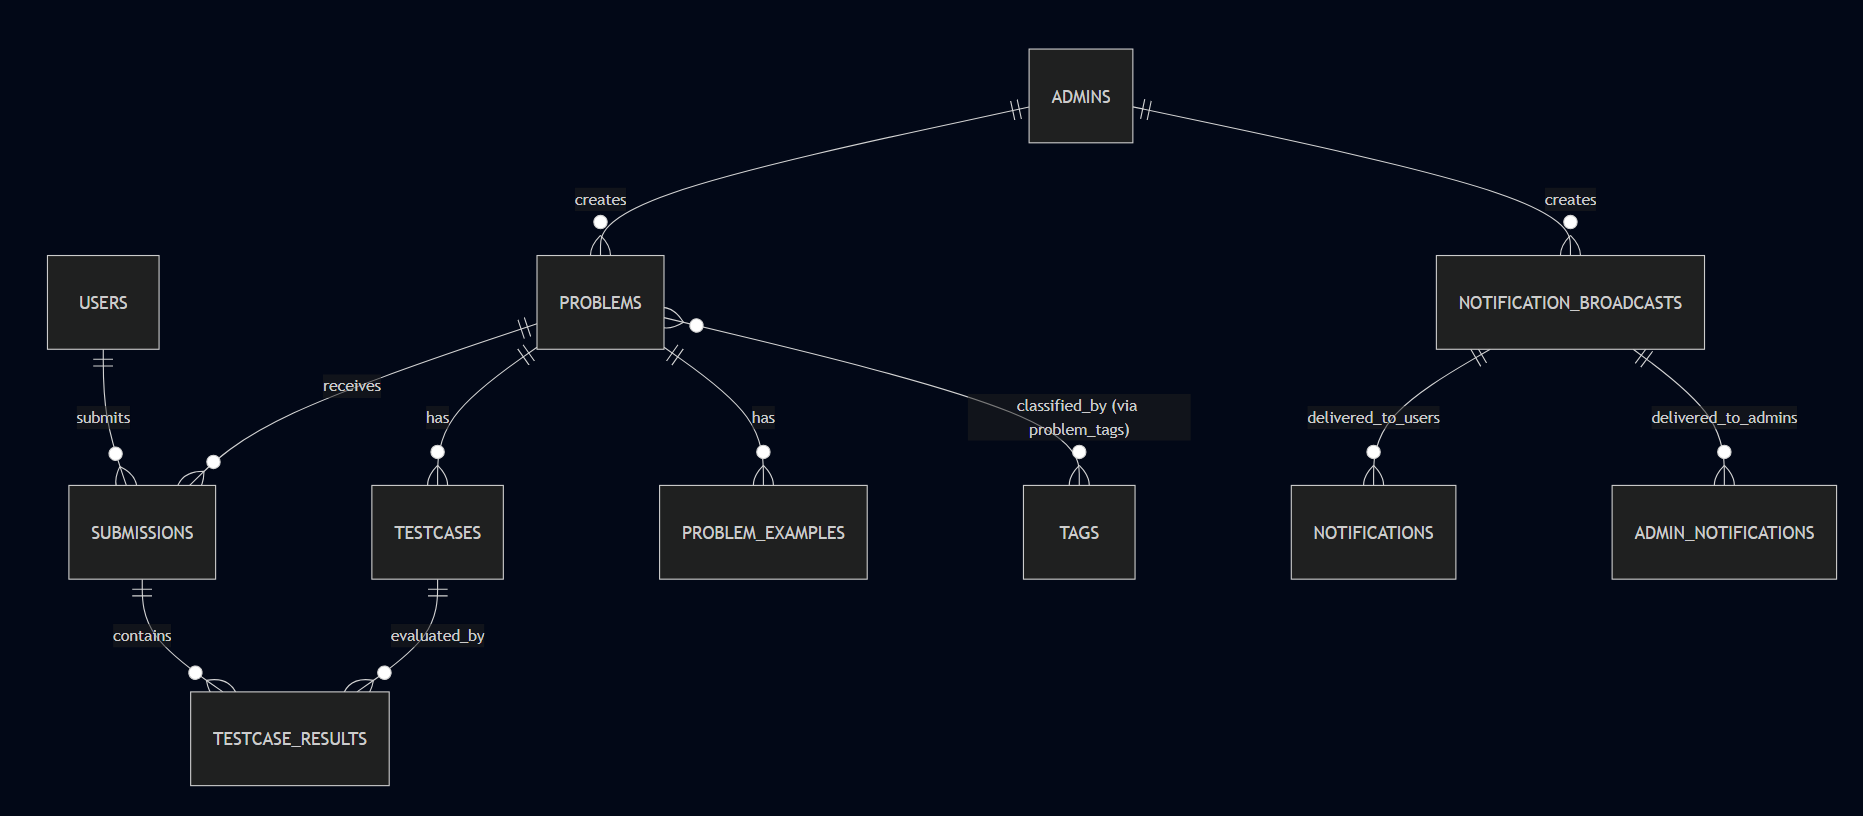
\includegraphics[
        width=\linewidth,
        height=0.85\textheight,
        keepaspectratio
    ]{pic/sodo_mqh_dulieu.png}
    \caption{So do moi quan he du lieu ERD}
\end{figure}

\subsection{4. Chiến lược lập chỉ mục tối ưu hiệu năng (Database Indexing Blueprint)}

Để đảm bảo hệ thống không xảy ra tình trạng nghẽn hàng đợi kết nối (Database Connection Pool Starvation) khi có hàng ngàn yêu cầu nộp bài cùng lúc, các chỉ mục (Indexes) sau được thiết lập dựa trên tần suất truy vấn thực tế của các API.

\subsubsection{4.1. Xác thực \& Tìm kiếm tài khoản}

\begin{Shaded}
\begin{Highlighting}[]
\CommentTok{{-}{-} Đẩy nhanh tốc độ kiểm tra khi Đăng nhập và hiển thị Profile}
\KeywordTok{CREATE} \KeywordTok{UNIQUE} \KeywordTok{INDEX}\NormalTok{ idx\_users\_username }\KeywordTok{ON}\NormalTok{ users(username);}

\CommentTok{{-}{-} Tối ưu hóa luồng Đăng ký tài khoản và khôi phục mật khẩu}
\KeywordTok{CREATE} \KeywordTok{UNIQUE} \KeywordTok{INDEX}\NormalTok{ idx\_users\_email }\KeywordTok{ON}\NormalTok{ users(email);}

\CommentTok{{-}{-} Xác thực tài khoản quản trị viên tốc độ cao}
\KeywordTok{CREATE} \KeywordTok{UNIQUE} \KeywordTok{INDEX}\NormalTok{ idx\_admins\_credential }\KeywordTok{ON}\NormalTok{ admins(username, email);}
\end{Highlighting}
\end{Shaded}

\subsubsection{4.2. Bảng xếp hạng (Leaderboard)}

\begin{Shaded}
\begin{Highlighting}[]
\CommentTok{{-}{-} Lọc danh sách học viên tích cực, không cần Full Table Scan}
\KeywordTok{CREATE} \KeywordTok{INDEX}\NormalTok{ idx\_users\_leaderboard }\KeywordTok{ON}\NormalTok{ users(is\_active, deleted\_at, total\_score }\KeywordTok{DESC}\NormalTok{);}
\end{Highlighting}
\end{Shaded}

\subsubsection{4.3. Tìm kiếm Bài tập (Problems Discovery)}

\begin{Shaded}
\begin{Highlighting}[]
\CommentTok{{-}{-} Lọc danh sách bài tập theo độ khó ở màn hình trang chủ}
\KeywordTok{CREATE} \KeywordTok{INDEX}\NormalTok{ idx\_problems\_filter }\KeywordTok{ON}\NormalTok{ problems(is\_public, difficulty);}

\CommentTok{{-}{-} Hiển thị danh sách các bài tập mới nhất}
\KeywordTok{CREATE} \KeywordTok{INDEX}\NormalTok{ idx\_problems\_latest }\KeywordTok{ON}\NormalTok{ problems(is\_public, created\_at }\KeywordTok{DESC}\NormalTok{);}

\CommentTok{{-}{-} Tìm kiếm bài tập theo từ khóa không phân biệt hoa/thường}
\KeywordTok{CREATE} \KeywordTok{INDEX}\NormalTok{ idx\_problems\_title\_lower }\KeywordTok{ON}\NormalTok{ problems(}\FunctionTok{LOWER}\NormalTok{(title));}
\end{Highlighting}
\end{Shaded}

\subsubsection{4.4. Chấm bài \& Lịch sử hệ thống (Submissions Management)}

\begin{Shaded}
\begin{Highlighting}[]
\CommentTok{{-}{-} Hiển thị trang "Lịch sử nộp bài cá nhân" của học viên}
\KeywordTok{CREATE} \KeywordTok{INDEX}\NormalTok{ idx\_submissions\_user }\KeywordTok{ON}\NormalTok{ submissions(user\_id, submitted\_at }\KeywordTok{DESC}\NormalTok{);}

\CommentTok{{-}{-} Hiển thị trang "Lịch sử giải bài" của một bài toán cụ thể}
\KeywordTok{CREATE} \KeywordTok{INDEX}\NormalTok{ idx\_submissions\_problem }\KeywordTok{ON}\NormalTok{ submissions(problem\_id, submitted\_at }\KeywordTok{DESC}\NormalTok{);}

\CommentTok{{-}{-} Hỗ trợ Judge Engine truy vấn kết quả chi tiết theo Submission}
\KeywordTok{CREATE} \KeywordTok{INDEX}\NormalTok{ idx\_testcase\_results\_lookup }\KeywordTok{ON}\NormalTok{ testcase\_results(submission\_id, testcase\_id);}
\end{Highlighting}
\end{Shaded}

\subsubsection{4.5. Truyền tải Thông báo (Notifications Polling)}

\begin{Shaded}
\begin{Highlighting}[]
\CommentTok{{-}{-} Tối ưu API Polling đếm số thông báo chưa đọc trên thanh điều hướng}
\KeywordTok{CREATE} \KeywordTok{INDEX}\NormalTok{ idx\_notifications\_user\_unread }\KeywordTok{ON}\NormalTok{ notifications(user\_id, is\_read, created\_at }\KeywordTok{DESC}\NormalTok{);}
\end{Highlighting}
\end{Shaded}

\subsection{5. Ghi chú thiết kế hệ thống dữ liệu (Design Notes)}

Để tối ưu hóa toàn diện cho một hệ thống Online Judge thực tế, cấu trúc cơ sở dữ liệu của ByeBug áp dụng các nguyên lý thiết kế đặc thù sau:

\begin{itemize}
\item
  \textbf{Cơ chế Xóa mềm (Soft Delete) ổn định lịch sử:} Bảng \texttt{users} sử dụng cặp trường \texttt{is\_active} và \texttt{deleted\_at} thay vì lệnh xóa cứng (\texttt{DELETE}). Thiết kế này giúp bảo toàn tính toàn vẹn dữ liệu (Data Integrity). Khi một tài khoản bị xóa, toàn bộ lịch sử nộp bài (\texttt{submissions}) của họ vẫn được giữ lại để làm tài nguyên thống kê hệ thống và không làm lỗi các liên kết khóa ngoại.
\item
  \textbf{Mô hình Lưu trữ hỗn hợp tối ưu tài nguyên (Hybrid Storage Engine):} Toàn bộ dữ liệu kiểm thử nặng (Testcases) không lưu trực tiếp dưới dạng Binary (BLOB) trong PostgreSQL để tránh tình trạng phân mảnh và phình to dữ liệu đĩa cứng. Database chỉ lưu các Object Key độc lập; việc đọc/ghi file vật lý được nhường lại cho MinIO để đạt hiệu suất IOPS tối đa.
\item
  \textbf{Quan hệ Nhiều-Nhiều linh hoạt cho bài tập:} Thiết kế bảng trung gian \texttt{problem\_tags} kết nối giữa \texttt{problems} và \texttt{tags} giúp một bài toán có thể thuộc nhiều chủ đề thuật toán khác nhau (Ví dụ: một bài vừa thuộc tag \emph{Array}, vừa thuộc tag \emph{Two Pointers}), hỗ trợ bộ lọc phía Frontend hoạt động chính xác và đa dạng.
\item
  \textbf{Tách biệt Submission và Testcase Result:} Việc tách thành hai bảng độc lập cho phép hệ thống ghi nhận chi tiết kết quả chạy (thời gian, bộ nhớ, kết quả lỗi) của \textbf{từng Testcase một} thay vì chỉ lưu kết quả tổng quan. Đây là cơ sở dữ liệu cốt lõi để hiển thị giao diện xem tiến trình chấm bài trực quan cho học viên.
\item
  \textbf{Tách biệt Tài khoản Quản trị nội bộ:} Tách bảng \texttt{admins} độc lập hoàn toàn với bảng \texttt{users} giúp cô lập phân vùng dữ liệu, tăng cường bảo mật tầng cơ sở dữ liệu và ngăn chặn các cuộc tấn công leo thang đặc quyền (Privilege Escalation).
\end{itemize}

\newpage

\section{CHƯƠNG 3. Đặc tả hệ thống REST API ByeBug}

\subsection{1. Quy ước chung}

Mọi tương tác truyền tải dữ liệu giữa môi trường Frontend (React) và Backend (Spring Boot) của hệ thống ByeBug được đóng gói đồng bộ thông qua giao thức \textbf{HTTP/HTTPS} với định dạng gói tin cấu trúc \textbf{JSON}.

\begin{itemize}
\tightlist
\item
  \textbf{Cấu hình Base URL vật lý (Localhost):} \texttt{http://localhost:8080/api}
\item
  \textbf{Quy ước Header dành cho các API yêu cầu xác thực (Protected APIs):}
\end{itemize}

\begin{Shaded}
\begin{Highlighting}[]
\NormalTok{Authorization: Bearer \textless{}access\_token\textgreater{}}
\NormalTok{Content{-}Type: application/json}
\end{Highlighting}
\end{Shaded}

\begin{itemize}
\tightlist
\item
  \textbf{Quy ước cấu trúc phản hồi lỗi hệ thống (Standard Error Response):} Để tăng tính đồng bộ và dễ dàng bóc tách thông tin tại tầng Frontend, toàn bộ lỗi xử lý nghiệp vụ hoặc lỗi hệ thống được đóng gói theo cấu trúc:
\end{itemize}

\begin{Shaded}
\begin{Highlighting}[]
\FunctionTok{\{}
  \DataTypeTok{"timestamp"}\FunctionTok{:} \StringTok{"2026{-}06{-}13T12:30:00.123Z"}\FunctionTok{,}
  \DataTypeTok{"status"}\FunctionTok{:} \DecValTok{400}\FunctionTok{,}
  \DataTypeTok{"error"}\FunctionTok{:} \StringTok{"Bad Request"}\FunctionTok{,}
  \DataTypeTok{"message"}\FunctionTok{:} \StringTok{"Chi tiết nguyên nhân gây lỗi hệ thống."}\FunctionTok{,}
  \DataTypeTok{"path"}\FunctionTok{:} \StringTok{"/api/v1/resource{-}path"}
\FunctionTok{\}}
\end{Highlighting}
\end{Shaded}

\subsection{2. Phân hệ API dành cho Học viên (Auth \& Users APIs)}

Base Path: \texttt{/api/users}

\begin{longtable}[]{
  |>{\raggedright\arraybackslash}p{(\linewidth - 10\tabcolsep) * \real{0.2500}}
  |>{\raggedright\arraybackslash}p{(\linewidth - 10\tabcolsep) * \real{0.2500}}
  |>{\raggedright\arraybackslash}p{(\linewidth - 10\tabcolsep) * \real{0.2500}}
  |>{\raggedright\arraybackslash}p{(\linewidth - 10\tabcolsep) * \real{0.2500}}|}
\hline\rowcolor{tableHeader}
\begin{minipage}[b]{\linewidth}\raggedright
Phương thức
\end{minipage} & \begin{minipage}[b]{\linewidth}\raggedright
Đường dẫn Endpoint
\end{minipage} & \begin{minipage}[b]{\linewidth}\raggedright
Nghiệp vụ chức năng
\end{minipage} & \begin{minipage}[b]{\linewidth}\raggedright
Trạng thái bảo mật
\end{minipage} \\
\hline
\endhead
\hline
\endlastfoot
POST & \texttt{/register} & Đăng ký tài khoản học viên mới. & Public \\
\hline
POST & \texttt{/login} & Đăng nhập tài khoản vào hệ thống. & Public \\
\hline
POST & \texttt{/forgot-password} & Yêu cầu gửi mã khôi phục mật khẩu. & Public \\
\hline
GET & \texttt{/\{username\}} & Truy vấn chi tiết hồ sơ (Profile) người dùng. & Học viên / Admin \\
\hline
GET & \texttt{/leaderboard} & Truy vấn bảng xếp hạng học viên theo tổng điểm. & Public \\
\hline
GET & \tablecelllines{\texttt{/statistics/}\\\texttt{\{username\}}} & Truy vấn số liệu thống kê học tập cá nhân. & Học viên / Admin \\
\hline
PUT & \texttt{/\{username\}} & Cập nhật thông tin cá nhân. & Học viên \\
\hline
POST & \tablecelllines{\texttt{/change-password/}\\\texttt{\{username\}}} & Thực hiện đổi mật khẩu tài khoản. & Học viên \\
\hline
DELETE & \texttt{/\{username\}} & Yêu cầu xóa tài khoản (Soft Delete). & Học viên / Admin \\
\hline
\end{longtable}

\subsubsection{\texorpdfstring{2.1. API: Đăng ký tài khoản (\texttt{POST\ /api/users/register})}{2.1. API: Đăng ký tài khoản (POST /api/users/register)}}

\textbf{Request Body:}

\begin{Shaded}
\begin{Highlighting}[]
\FunctionTok{\{}
  \DataTypeTok{"username"}\FunctionTok{:} \StringTok{"student2452"}\FunctionTok{,}
  \DataTypeTok{"fullName"}\FunctionTok{:} \StringTok{"Nguyễn Ngọc Thu An"}\FunctionTok{,}
  \DataTypeTok{"email"}\FunctionTok{:} \StringTok{"an.nn@uit.edu.vn"}\FunctionTok{,}
  \DataTypeTok{"password"}\FunctionTok{:} \StringTok{"SecurePassword123"}
\FunctionTok{\}}
\end{Highlighting}
\end{Shaded}

\textbf{Response (201 Created):}

\begin{Shaded}
\begin{Highlighting}[]
\FunctionTok{\{}
  \DataTypeTok{"userId"}\FunctionTok{:} \DecValTok{24520063}\FunctionTok{,}
  \DataTypeTok{"username"}\FunctionTok{:} \StringTok{"student2452"}\FunctionTok{,}
  \DataTypeTok{"fullName"}\FunctionTok{:} \StringTok{"Nguyễn Ngọc Thu An"}\FunctionTok{,}
  \DataTypeTok{"email"}\FunctionTok{:} \StringTok{"an.nn@uit.edu.vn"}\FunctionTok{,}
  \DataTypeTok{"role"}\FunctionTok{:} \StringTok{"USER"}\FunctionTok{,}
  \DataTypeTok{"totalScore"}\FunctionTok{:} \DecValTok{0}\FunctionTok{,}
  \DataTypeTok{"createdAt"}\FunctionTok{:} \StringTok{"2026{-}06{-}13T12:31:00Z"}
\FunctionTok{\}}
\end{Highlighting}
\end{Shaded}

\subsubsection{\texorpdfstring{2.2. API: Đăng nhập hệ thống (\texttt{POST\ /api/users/login})}{2.2. API: Đăng nhập hệ thống (POST /api/users/login)}}

\textbf{Request Body:}

\begin{Shaded}
\begin{Highlighting}[]
\FunctionTok{\{}
  \DataTypeTok{"usernameOrEmail"}\FunctionTok{:} \StringTok{"student2452"}\FunctionTok{,}
  \DataTypeTok{"password"}\FunctionTok{:} \StringTok{"SecurePassword123"}
\FunctionTok{\}}
\end{Highlighting}
\end{Shaded}

\textbf{Response (200 OK):}

\begin{Shaded}
\begin{Highlighting}[]
\FunctionTok{\{}
  \DataTypeTok{"token"}\FunctionTok{:} \StringTok{"eyJhbGciOiJIUzI1NiIsInR5cCI6IkpXVCJ9..."}\FunctionTok{,}
  \DataTypeTok{"expiresIn"}\FunctionTok{:} \DecValTok{86400}\FunctionTok{,}
  \DataTypeTok{"user"}\FunctionTok{:} \FunctionTok{\{}
    \DataTypeTok{"userId"}\FunctionTok{:} \DecValTok{24520063}\FunctionTok{,}
    \DataTypeTok{"username"}\FunctionTok{:} \StringTok{"student2452"}\FunctionTok{,}
    \DataTypeTok{"fullName"}\FunctionTok{:} \StringTok{"Nguyễn Ngọc Thu An"}\FunctionTok{,}
    \DataTypeTok{"role"}\FunctionTok{:} \StringTok{"USER"}
  \FunctionTok{\}}
\FunctionTok{\}}
\end{Highlighting}
\end{Shaded}

\subsection{3. Phân hệ API Quản trị phân quyền (Admin Auth API)}

Base Path: \texttt{/api/admin}

\begin{longtable}[]{
  |>{\raggedright\arraybackslash}p{(\linewidth - 10\tabcolsep) * \real{0.2500}}
  |>{\raggedright\arraybackslash}p{(\linewidth - 10\tabcolsep) * \real{0.2500}}
  |>{\raggedright\arraybackslash}p{(\linewidth - 10\tabcolsep) * \real{0.2500}}
  |>{\raggedright\arraybackslash}p{(\linewidth - 10\tabcolsep) * \real{0.2500}}|}
\hline\rowcolor{tableHeader}
\begin{minipage}[b]{\linewidth}\raggedright
Phương thức
\end{minipage} & \begin{minipage}[b]{\linewidth}\raggedright
Đường dẫn Endpoint
\end{minipage} & \begin{minipage}[b]{\linewidth}\raggedright
Nghiệp vụ chức năng
\end{minipage} & \begin{minipage}[b]{\linewidth}\raggedright
Trạng thái bảo mật
\end{minipage} \\
\hline
\endhead
\hline
\endlastfoot
POST & \texttt{/login} & Đăng nhập dành riêng cho phân hệ Admin. & Public \\
\hline
GET & \texttt{/health} & Kiểm tra trạng thái hoạt động của hệ thống. & Public / Admin \\
\hline
\end{longtable}

\subsection{4. Phân hệ API Bài tập công khai (User Problem APIs)}

Base Path: \texttt{/api/problems}

\begin{longtable}[]{
  |>{\raggedright\arraybackslash}p{(\linewidth - 10\tabcolsep) * \real{0.2500}}
  |>{\raggedright\arraybackslash}p{(\linewidth - 10\tabcolsep) * \real{0.2500}}
  |>{\raggedright\arraybackslash}p{(\linewidth - 10\tabcolsep) * \real{0.2500}}
  |>{\raggedright\arraybackslash}p{(\linewidth - 10\tabcolsep) * \real{0.2500}}|}
\hline\rowcolor{tableHeader}
\begin{minipage}[b]{\linewidth}\raggedright
Phương thức
\end{minipage} & \begin{minipage}[b]{\linewidth}\raggedright
Đường dẫn Endpoint
\end{minipage} & \begin{minipage}[b]{\linewidth}\raggedright
Nghiệp vụ chức năng
\end{minipage} & \begin{minipage}[b]{\linewidth}\raggedright
Trạng thái bảo mật
\end{minipage} \\
\hline
\endhead
\hline
\endlastfoot
GET & \texttt{/} & Lấy danh sách bài tập hiển thị công khai (Có phân trang). & Public \\
\hline
GET & \texttt{/\{id\}} & Truy vấn chi tiết đề bài, ví dụ mẫu và giới hạn. & Public \\
\hline
GET & \tablecelllines{\texttt{/difficulty/}\\\texttt{\{difficulty\}}} & Lọc nhanh danh sách bài tập theo cấp độ khó. & Public \\
\hline
GET & \texttt{/search} & Tìm kiếm bài tập theo từ khóa tiêu đề hoặc thẻ Tag. & Public \\
\hline
\end{longtable}

\subsubsection{\texorpdfstring{4.1. API: Lấy danh sách bài tập công khai (\texttt{GET\ /api/problems})}{4.1. API: Lấy danh sách bài tập công khai (GET /api/problems)}}

Query Parameters: \texttt{page=0}, \texttt{size=10}

\textbf{Response (200 OK):}

\begin{Shaded}
\begin{Highlighting}[]
\FunctionTok{\{}
  \DataTypeTok{"content"}\FunctionTok{:} \OtherTok{[}
    \FunctionTok{\{}
      \DataTypeTok{"problemId"}\FunctionTok{:} \DecValTok{1}\FunctionTok{,}
      \DataTypeTok{"title"}\FunctionTok{:} \StringTok{"Two Sum"}\FunctionTok{,}
      \DataTypeTok{"difficulty"}\FunctionTok{:} \StringTok{"EASY"}\FunctionTok{,}
      \DataTypeTok{"timeLimitMs"}\FunctionTok{:} \DecValTok{2000}\FunctionTok{,}
      \DataTypeTok{"memoryLimitKb"}\FunctionTok{:} \DecValTok{262144}\FunctionTok{,}
      \DataTypeTok{"tags"}\FunctionTok{:} \OtherTok{[}\StringTok{"Array"}\OtherTok{,} \StringTok{"Hash Table"}\OtherTok{]}
    \FunctionTok{\}}
  \OtherTok{]}\FunctionTok{,}
  \DataTypeTok{"page"}\FunctionTok{:} \DecValTok{0}\FunctionTok{,}
  \DataTypeTok{"size"}\FunctionTok{:} \DecValTok{10}\FunctionTok{,}
  \DataTypeTok{"totalElements"}\FunctionTok{:} \DecValTok{1}\FunctionTok{,}
  \DataTypeTok{"totalPages"}\FunctionTok{:} \DecValTok{1}\FunctionTok{,}
  \DataTypeTok{"last"}\FunctionTok{:} \KeywordTok{true}
\FunctionTok{\}}
\end{Highlighting}
\end{Shaded}

\subsubsection{\texorpdfstring{4.2. API: Xem chi tiết đề bài tập (\texttt{GET\ /api/problems/\{id\}})}{4.2. API: Xem chi tiết đề bài tập (GET /api/problems/\{id\})}}

\textbf{Response (200 OK):}

\begin{Shaded}
\begin{Highlighting}[]
\FunctionTok{\{}
  \DataTypeTok{"problemId"}\FunctionTok{:} \DecValTok{1}\FunctionTok{,}
  \DataTypeTok{"title"}\FunctionTok{:} \StringTok{"Two Sum"}\FunctionTok{,}
  \DataTypeTok{"description"}\FunctionTok{:} \StringTok{"Cho một mảng số nguyên \textasciigrave{}nums\textasciigrave{} và một số nguyên \textasciigrave{}target\textasciigrave{}..."}\FunctionTok{,}
  \DataTypeTok{"constraints"}\FunctionTok{:} \StringTok{"2 \textless{}= nums.length \textless{}= 10\^{}4"}\FunctionTok{,}
  \DataTypeTok{"difficulty"}\FunctionTok{:} \StringTok{"EASY"}\FunctionTok{,}
  \DataTypeTok{"timeLimitMs"}\FunctionTok{:} \DecValTok{2000}\FunctionTok{,}
  \DataTypeTok{"memoryLimitKb"}\FunctionTok{:} \DecValTok{262144}\FunctionTok{,}
  \DataTypeTok{"allowFileSubmit"}\FunctionTok{:} \KeywordTok{false}\FunctionTok{,}
  \DataTypeTok{"tags"}\FunctionTok{:} \OtherTok{[}\StringTok{"Array"}\OtherTok{,} \StringTok{"Hash Table"}\OtherTok{]}\FunctionTok{,}
  \DataTypeTok{"examples"}\FunctionTok{:} \OtherTok{[}
    \FunctionTok{\{}
      \DataTypeTok{"input"}\FunctionTok{:} \StringTok{"4}\CharTok{\textbackslash{}n}\StringTok{2 7 11 15}\CharTok{\textbackslash{}n}\StringTok{9"}\FunctionTok{,}
      \DataTypeTok{"output"}\FunctionTok{:} \StringTok{"0 1"}\FunctionTok{,}
      \DataTypeTok{"explanation"}\FunctionTok{:} \StringTok{"Vì nums[0] + nums[1] == 9, ta trả về index 0 và 1."}\FunctionTok{,}
      \DataTypeTok{"displayOrder"}\FunctionTok{:} \DecValTok{1}
    \FunctionTok{\}}
  \OtherTok{]}
\FunctionTok{\}}
\end{Highlighting}
\end{Shaded}

\subsection{5. Phân hệ API Lượt nộp bài (Submission APIs)}

Base Path: \texttt{/api/submissions}

\begin{longtable}[]{
  |>{\raggedright\arraybackslash}p{(\linewidth - 10\tabcolsep) * \real{0.2500}}
  |>{\raggedright\arraybackslash}p{(\linewidth - 10\tabcolsep) * \real{0.2500}}
  |>{\raggedright\arraybackslash}p{(\linewidth - 10\tabcolsep) * \real{0.2500}}
  |>{\raggedright\arraybackslash}p{(\linewidth - 10\tabcolsep) * \real{0.2500}}|}
\hline\rowcolor{tableHeader}
\begin{minipage}[b]{\linewidth}\raggedright
Phương thức
\end{minipage} & \begin{minipage}[b]{\linewidth}\raggedright
Đường dẫn Endpoint
\end{minipage} & \begin{minipage}[b]{\linewidth}\raggedright
Nghiệp vụ chức năng
\end{minipage} & \begin{minipage}[b]{\linewidth}\raggedright
Trạng thái bảo mật
\end{minipage} \\
\hline
\endhead
\hline
\endlastfoot
POST & \texttt{/} & Gửi mã nguồn bài giải lên hệ thống (Nộp bài). & Học viên \\
\hline
GET & \texttt{/\{submissionId\}} & Truy vấn kết quả chấm chi tiết của một lượt nộp. & Học viên / Admin \\
\hline
GET & \texttt{/admin} & Truy vấn toàn bộ danh sách lượt nộp hệ thống. & Admin \\
\hline
PATCH & \tablecelllines{\texttt{/admin/}\\\texttt{\{submissionId\}/}\\\texttt{rejudge}} & Yêu cầu Judge Engine chấm lại bài làm chỉ định. & Admin \\
\hline
PATCH & \tablecelllines{\texttt{/admin/}\\\texttt{\{submissionId\}/}\\\texttt{accept}} & Cưỡng chế công nhận bài làm đúng bằng tay. & Admin \\
\hline
\end{longtable}

\subsubsection{\texorpdfstring{5.1. API: Gửi mã nguồn nộp bài (\texttt{POST\ /api/submissions})}{5.1. API: Gửi mã nguồn nộp bài (POST /api/submissions)}}

\textbf{Request Body:}

\begin{Shaded}
\begin{Highlighting}[]
\FunctionTok{\{}
  \DataTypeTok{"problemId"}\FunctionTok{:} \DecValTok{1}\FunctionTok{,}
  \DataTypeTok{"language"}\FunctionTok{:} \StringTok{"CPP"}\FunctionTok{,}
  \DataTypeTok{"sourceCode"}\FunctionTok{:} \StringTok{"\#include \textless{}bits/stdc++.h\textgreater{}}\CharTok{\textbackslash{}n}\StringTok{using namespace std;}\CharTok{\textbackslash{}n}\StringTok{int main() \{ return 0; \}"}
\FunctionTok{\}}
\end{Highlighting}
\end{Shaded}

\textbf{Response (202 Accepted):} Ghi nhận bài nộp thành công, chờ xếp lịch chấm bất đồng bộ.

\begin{Shaded}
\begin{Highlighting}[]
\FunctionTok{\{}
  \DataTypeTok{"submissionId"}\FunctionTok{:} \DecValTok{1001}\FunctionTok{,}
  \DataTypeTok{"problemId"}\FunctionTok{:} \DecValTok{1}\FunctionTok{,}
  \DataTypeTok{"language"}\FunctionTok{:} \StringTok{"CPP"}\FunctionTok{,}
  \DataTypeTok{"verdict"}\FunctionTok{:} \StringTok{"PENDING"}\FunctionTok{,}
  \DataTypeTok{"score"}\FunctionTok{:} \DecValTok{0}\FunctionTok{,}
  \DataTypeTok{"submittedAt"}\FunctionTok{:} \StringTok{"2026{-}06{-}13T10:00:00Z"}
\FunctionTok{\}}
\end{Highlighting}
\end{Shaded}

\subsubsection{\texorpdfstring{5.2. API: Xem kết quả chấm bài (\texttt{GET\ /api/submissions/\{submissionId\}})}{5.2. API: Xem kết quả chấm bài (GET /api/submissions/\{submissionId\})}}

\textbf{Response (200 OK):}

\begin{Shaded}
\begin{Highlighting}[]
\FunctionTok{\{}
  \DataTypeTok{"submissionId"}\FunctionTok{:} \DecValTok{1001}\FunctionTok{,}
  \DataTypeTok{"verdict"}\FunctionTok{:} \StringTok{"ACCEPTED"}\FunctionTok{,}
  \DataTypeTok{"score"}\FunctionTok{:} \DecValTok{100}\FunctionTok{,}
  \DataTypeTok{"totalTimeMs"}\FunctionTok{:} \DecValTok{120}\FunctionTok{,}
  \DataTypeTok{"maxMemoryKb"}\FunctionTok{:} \DecValTok{2048}\FunctionTok{,}
  \DataTypeTok{"compileError"}\FunctionTok{:} \KeywordTok{null}\FunctionTok{,}
  \DataTypeTok{"judgeMessage"}\FunctionTok{:} \StringTok{"All testcases passed successfully."}\FunctionTok{,}
  \DataTypeTok{"testcaseResults"}\FunctionTok{:} \OtherTok{[}
    \FunctionTok{\{}
      \DataTypeTok{"testcaseId"}\FunctionTok{:} \DecValTok{1}\FunctionTok{,}
      \DataTypeTok{"verdict"}\FunctionTok{:} \StringTok{"ACCEPTED"}\FunctionTok{,}
      \DataTypeTok{"timeMs"}\FunctionTok{:} \DecValTok{10}\FunctionTok{,}
      \DataTypeTok{"memoryKb"}\FunctionTok{:} \DecValTok{512}
    \FunctionTok{\}}
  \OtherTok{]}
\FunctionTok{\}}
\end{Highlighting}
\end{Shaded}

\subsection{6. Phân hệ API Quản trị bài tập dành cho Admin (Admin Problem APIs)}

Base Path: \texttt{/api/admin/problems}

\begin{longtable}[]{
  |>{\raggedright\arraybackslash}p{(\linewidth - 10\tabcolsep) * \real{0.2500}}
  |>{\raggedright\arraybackslash}p{(\linewidth - 10\tabcolsep) * \real{0.2500}}
  |>{\raggedright\arraybackslash}p{(\linewidth - 10\tabcolsep) * \real{0.2500}}
  |>{\raggedright\arraybackslash}p{(\linewidth - 10\tabcolsep) * \real{0.2500}}|}
\hline\rowcolor{tableHeader}
\begin{minipage}[b]{\linewidth}\raggedright
Phương thức
\end{minipage} & \begin{minipage}[b]{\linewidth}\raggedright
Đường dẫn Endpoint
\end{minipage} & \begin{minipage}[b]{\linewidth}\raggedright
Nghiệp vụ chức năng
\end{minipage} & \begin{minipage}[b]{\linewidth}\raggedright
Trạng thái bảo mật
\end{minipage} \\
\hline
\endhead
\hline
\endlastfoot
GET & \texttt{/} & Lấy toàn bộ danh sách bài toán hệ thống (Gồm bài ẩn). & Admin \\
\hline
GET & \texttt{/latest} & Lấy danh sách các bài tập vừa được biên soạn mới nhất. & Admin \\
\hline
GET & \texttt{/popular} & Lấy danh sách các bài tập có lượt làm nhiều nhất. & Admin \\
\hline
GET & \texttt{/\{problemId\}} & Truy vấn sâu thông tin cấu trúc nội bộ của bài toán. & Admin \\
\hline
POST & \texttt{/} & Khởi tạo một bài toán lập trình mới. & Admin \\
\hline
PUT & \texttt{/\{problemId\}} & Cập nhật thông tin/đề bài/cấu hình bài toán. & Admin \\
\hline
POST & \tablecelllines{\texttt{/\{problemId\}/}\\\texttt{tests}} & Tải tập tin Testcase dữ liệu kiểm thử lên hệ thống. & Admin \\
\hline
PATCH & \tablecelllines{\texttt{/\{problemId\}/}\\\texttt{visibility}} & Chuyển đổi trạng thái Ẩn/Hiện bài tập ra trang chủ. & Admin \\
\hline
\end{longtable}

\subsubsection{\texorpdfstring{6.1. API: Khởi tạo bài toán mới (\texttt{POST\ /api/admin/problems})}{6.1. API: Khởi tạo bài toán mới (POST /api/admin/problems)}}

\textbf{Request Body:}

\begin{Shaded}
\begin{Highlighting}[]
\FunctionTok{\{}
  \DataTypeTok{"title"}\FunctionTok{:} \StringTok{"Two Sum"}\FunctionTok{,}
  \DataTypeTok{"description"}\FunctionTok{:} \StringTok{"Given an array of integers..."}\FunctionTok{,}
  \DataTypeTok{"constraints"}\FunctionTok{:} \StringTok{"1 \textless{}= n \textless{}= 10\^{}5"}\FunctionTok{,}
  \DataTypeTok{"difficulty"}\FunctionTok{:} \StringTok{"EASY"}\FunctionTok{,}
  \DataTypeTok{"timeLimitMs"}\FunctionTok{:} \DecValTok{2000}\FunctionTok{,}
  \DataTypeTok{"memoryLimitKb"}\FunctionTok{:} \DecValTok{262144}\FunctionTok{,}
  \DataTypeTok{"allowFileSubmit"}\FunctionTok{:} \KeywordTok{false}\FunctionTok{,}
  \DataTypeTok{"isPublic"}\FunctionTok{:} \KeywordTok{false}\FunctionTok{,}
  \DataTypeTok{"tags"}\FunctionTok{:} \OtherTok{[}\StringTok{"Array"}\OtherTok{,} \StringTok{"Hash Table"}\OtherTok{]}\FunctionTok{,}
  \DataTypeTok{"examples"}\FunctionTok{:} \OtherTok{[}
    \FunctionTok{\{}
      \DataTypeTok{"input"}\FunctionTok{:} \StringTok{"4}\CharTok{\textbackslash{}n}\StringTok{2 7 11 15}\CharTok{\textbackslash{}n}\StringTok{9"}\FunctionTok{,}
      \DataTypeTok{"output"}\FunctionTok{:} \StringTok{"0 1"}\FunctionTok{,}
      \DataTypeTok{"explanation"}\FunctionTok{:} \StringTok{"2 + 7 = 9"}\FunctionTok{,}
      \DataTypeTok{"displayOrder"}\FunctionTok{:} \DecValTok{1}
    \FunctionTok{\}}
  \OtherTok{]}
\FunctionTok{\}}
\end{Highlighting}
\end{Shaded}

\subsection{7. Phân hệ API Quản lý Người dùng dành cho Admin (Admin User APIs)}

Base Path: \texttt{/api/admin/users}

\begin{longtable}[]{
  |>{\raggedright\arraybackslash}p{(\linewidth - 10\tabcolsep) * \real{0.2500}}
  |>{\raggedright\arraybackslash}p{(\linewidth - 10\tabcolsep) * \real{0.2500}}
  |>{\raggedright\arraybackslash}p{(\linewidth - 10\tabcolsep) * \real{0.2500}}
  |>{\raggedright\arraybackslash}p{(\linewidth - 10\tabcolsep) * \real{0.2500}}|}
\hline\rowcolor{tableHeader}
\begin{minipage}[b]{\linewidth}\raggedright
Phương thức
\end{minipage} & \begin{minipage}[b]{\linewidth}\raggedright
Đường dẫn Endpoint
\end{minipage} & \begin{minipage}[b]{\linewidth}\raggedright
Nghiệp vụ chức năng
\end{minipage} & \begin{minipage}[b]{\linewidth}\raggedright
Trạng thái bảo mật
\end{minipage} \\
\hline
\endhead
\hline
\endlastfoot
GET & \texttt{/} & Truy vấn danh sách toàn bộ người dùng hệ thống. & Admin \\
\hline
GET & \texttt{/top} & Truy vấn top học viên xuất sắc phục vụ thống kê. & Admin \\
\hline
PATCH & \texttt{/\{userId\}/active} & Thực hiện Khóa hoặc Mở khóa tài khoản học viên. & Admin \\
\hline
DELETE & \texttt{/\{userId\}} & Thực hiện xóa mềm (Soft Delete) tài khoản người dùng. & Admin \\
\hline
POST & \texttt{/\{userId\}/restore} & Khôi phục tài khoản đã bị xóa mềm trước đó. & Admin \\
\hline
\end{longtable}

\subsection{8. Phân hệ API Quản lý Thông báo (Notification APIs)}

\subsubsection{\texorpdfstring{8.1. Phân hệ dành cho Học viên (\texttt{/api/notifications})}{8.1. Phân hệ dành cho Học viên (/api/notifications)}}

\begin{longtable}[]{
  |>{\raggedright\arraybackslash}p{(\linewidth - 10\tabcolsep) * \real{0.2500}}
  |>{\raggedright\arraybackslash}p{(\linewidth - 10\tabcolsep) * \real{0.2500}}
  |>{\raggedright\arraybackslash}p{(\linewidth - 10\tabcolsep) * \real{0.2500}}
  |>{\raggedright\arraybackslash}p{(\linewidth - 10\tabcolsep) * \real{0.2500}}|}
\hline\rowcolor{tableHeader}
\begin{minipage}[b]{\linewidth}\raggedright
Phương thức
\end{minipage} & \begin{minipage}[b]{\linewidth}\raggedright
Đường dẫn Endpoint
\end{minipage} & \begin{minipage}[b]{\linewidth}\raggedright
Nghiệp vụ chức năng
\end{minipage} & \begin{minipage}[b]{\linewidth}\raggedright
Trạng thái bảo mật
\end{minipage} \\
\hline
\endhead
\hline
\endlastfoot
GET & \texttt{/} & Lấy danh sách thông báo được gửi đến tài khoản này. & Học viên \\
\hline
GET & \texttt{/unread-count} & Kiểm tra số lượng thông báo mới chưa đọc. & Học viên \\
\hline
PATCH & \texttt{/\{id\}/read} & Đánh dấu một thông báo cụ thể là đã đọc. & Học viên \\
\hline
\end{longtable}

\subsubsection{\texorpdfstring{8.2. Phân hệ dành cho Admin (\texttt{/api/admin/notifications})}{8.2. Phân hệ dành cho Admin (/api/admin/notifications)}}

\begin{longtable}[]{
  |>{\raggedright\arraybackslash}p{(\linewidth - 10\tabcolsep) * \real{0.2500}}
  |>{\raggedright\arraybackslash}p{(\linewidth - 10\tabcolsep) * \real{0.2500}}
  |>{\raggedright\arraybackslash}p{(\linewidth - 10\tabcolsep) * \real{0.2500}}
  |>{\raggedright\arraybackslash}p{(\linewidth - 10\tabcolsep) * \real{0.2500}}|}
\hline\rowcolor{tableHeader}
\begin{minipage}[b]{\linewidth}\raggedright
Phương thức
\end{minipage} & \begin{minipage}[b]{\linewidth}\raggedright
Đường dẫn Endpoint
\end{minipage} & \begin{minipage}[b]{\linewidth}\raggedright
Nghiệp vụ chức năng
\end{minipage} & \begin{minipage}[b]{\linewidth}\raggedright
Trạng thái bảo mật
\end{minipage} \\
\hline
\endhead
\hline
\endlastfoot
POST & \texttt{/} & Phát hành một thông báo Broadcast đến toàn hệ thống. & Admin \\
\hline
GET & \texttt{/} & Xem lịch sử các thông báo diện rộng đã phát hành. & Admin \\
\hline
GET & \texttt{/inbox} & Xem hộp thư thông báo hệ thống nội bộ của Admin. & Admin \\
\hline
PATCH & \texttt{/inbox/\{id\}/read} & Đánh dấu thông báo nội bộ của admin đã đọc. & Admin \\
\hline
GET & \tablecelllines{\texttt{/inbox/}\\\texttt{unread-count}} & Đếm số thông báo quản trị hệ thống chưa xác nhận. & Admin \\
\hline
\end{longtable}

\subsection{9. Phân hệ API Thống kê \& Dashboard (Home / Overview APIs)}

\begin{longtable}[]{
  |>{\raggedright\arraybackslash}p{(\linewidth - 10\tabcolsep) * \real{0.2500}}
  |>{\raggedright\arraybackslash}p{(\linewidth - 10\tabcolsep) * \real{0.2500}}
  |>{\raggedright\arraybackslash}p{(\linewidth - 10\tabcolsep) * \real{0.2500}}
  |>{\raggedright\arraybackslash}p{(\linewidth - 10\tabcolsep) * \real{0.2500}}|}
\hline\rowcolor{tableHeader}
\begin{minipage}[b]{\linewidth}\raggedright
Phương thức
\end{minipage} & \begin{minipage}[b]{\linewidth}\raggedright
Đường dẫn Endpoint
\end{minipage} & \begin{minipage}[b]{\linewidth}\raggedright
Nghiệp vụ chức năng
\end{minipage} & \begin{minipage}[b]{\linewidth}\raggedright
Trạng thái bảo mật
\end{minipage} \\
\hline
\endhead
\hline
\endlastfoot
GET & \texttt{/api/home/summary} & Lấy tổng quan thông tin trang chủ của Học viên. & Học viên \\
\hline
GET & \tablecelllines{\texttt{/api/admin/}\\\texttt{overview}} & Lấy các chỉ số biểu đồ Dashboard tổng quan Admin. & Admin \\
\hline
\end{longtable}

\subsection{10. Định nghĩa hệ thống mã trạng thái (Standard HTTP Status Codes)}

Hệ thống cam kết sử dụng các mã trạng thái tiêu chuẩn của giao thức HTTP để phản hồi kết quả:

\begin{longtable}[]{
  |>{\raggedright\arraybackslash}p{(\linewidth - 6\tabcolsep) * \real{0.5000}}
  |>{\raggedright\arraybackslash}p{(\linewidth - 6\tabcolsep) * \real{0.5000}}|}
\hline\rowcolor{tableHeader}
\begin{minipage}[b]{\linewidth}\raggedright
Mã
\end{minipage} & \begin{minipage}[b]{\linewidth}\raggedright
Ý nghĩa
\end{minipage} \\
\hline
\endhead
\hline
\endlastfoot
200 OK & Các yêu cầu đọc dữ liệu (GET), cập nhật (PUT/PATCH) hoặc xử lý nghiệp vụ thành công. \\
\hline
201 Created & Khởi tạo thành công các đối tượng thực thể mới (Users, Problems). \\
\hline
202 Accepted & Tiếp nhận gói tin thành công và xếp lịch xử lý ngầm (Áp dụng cho luồng nộp bài Submissions). \\
\hline
400 Bad Request & Cấu trúc gói tin JSON gửi lên bị sai cú pháp, thiếu trường bắt buộc hoặc sai định dạng dữ liệu. \\
\hline
401 Unauthorized & Token đính kèm bị hết hạn, không hợp lệ hoặc người dùng chưa thực hiện đăng nhập. \\
\hline
403 Forbidden & Tài khoản học viên cố tình gọi các API thuộc đặc quyền Quản trị viên (\texttt{/api/admin/}). \\
\hline
404 Not Found & Tài nguyên yêu cầu (Bài tập, Lượt nộp bài, Tài khoản) không tồn tại trên hệ thống. \\
\hline
409 Conflict & Xảy ra xung đột tài nguyên dữ liệu hệ thống (Trùng lặp tên \texttt{username} hoặc địa chỉ \texttt{email}). \\
\hline
500 Internal Server Error & Lỗi phát sinh ngoài dự kiến xuất phát từ mã nguồn máy chủ. \\
\hline
\end{longtable}

\newpage

\section{CHƯƠNG 4. Kiến trúc thành phần và triển khai hệ thống ByeBug}

\subsection{1. Môi trường công nghệ nền tảng (Technology Stack)}

Hệ thống ByeBug được đóng gói và vận hành dựa trên sự phối hợp của các công nghệ hiện đại, đảm bảo tính bất đồng bộ và khả năng chịu tải tốt:

\begin{longtable}[]{
  |>{\raggedright\arraybackslash}p{(\linewidth - 8\tabcolsep) * \real{0.3333}}
  |>{\raggedright\arraybackslash}p{(\linewidth - 8\tabcolsep) * \real{0.3333}}
  |>{\raggedright\arraybackslash}p{(\linewidth - 8\tabcolsep) * \real{0.3333}}|}
\hline\rowcolor{tableHeader}
\begin{minipage}[b]{\linewidth}\raggedright
Tầng chức năng
\end{minipage} & \begin{minipage}[b]{\linewidth}\raggedright
Công nghệ sử dụng
\end{minipage} & \begin{minipage}[b]{\linewidth}\raggedright
Vai trò chi tiết
\end{minipage} \\
\hline
\endhead
\hline
\endlastfoot
\textbf{Presentation (Frontend)} & React 19, TypeScript, Vite, React Router, Axios, Monaco Editor, Recharts & Xây dựng giao diện Single Page Application (SPA), tích hợp trình soạn thảo code thông minh và hệ thống biểu đồ trực quan. \\
\hline
\textbf{Business Logic (Backend)} & Java Spring Boot, Spring MVC, Spring Security, JWT, Spring Data JPA, Hibernate & Xử lý toàn bộ logic nghiệp vụ hệ thống, quản lý phiên xác thực, phân quyền endpoint. \\
\hline
\textbf{Execution (Judge Engine)} & Java Spring Boot Worker, Redis Consumer, Docker Java API & Khối xử lý ngầm tiêu thụ tác vụ chấm bài, tương tác với hạ tầng ảo hóa để chạy mã nguồn người dùng. \\
\hline
\textbf{Relational Database} & PostgreSQL 17 & Lưu trữ dữ liệu quan hệ có tính toàn vẹn cao (Users, Problems, Submissions). \\
\hline
\textbf{Cache \& Message Broker} & Redis 7 & Tầng đệm tối ưu truy vấn dữ liệu và đóng vai trò hàng đợi phân phối tác vụ (Job Queue). \\
\hline
\textbf{Object Storage} & MinIO (S3 Compatible) & Kho lưu trữ tệp tin Testcase cô lập, giải tải dung lượng lưu trữ cho Database chính. \\
\hline
\textbf{Virtualization} & Docker, Docker Compose & Đóng gói môi trường, cô lập tài nguyên phần cứng và điều phối các dịch vụ. \\
\hline
\end{longtable}

\subsection{2. Cấu trúc tổ chức mã nguồn (Source Code Directory Tree)}

Mã nguồn dự án ByeBug được tổ chức theo kiến trúc Monorepo giúp quản lý tập trung và đồng bộ hóa biến môi trường cấu hình một cách dễ dàng:

\begin{Shaded}
\begin{Highlighting}[]
\NormalTok{ByeBug{-}main/}
\NormalTok{├── frontend/               \# Ứng dụng giao diện người dùng UI (React + TypeScript)}
\NormalTok{├── backend/                \# Ứng dụng cung cấp các dịch vụ RESTful API (Spring Boot)}
\NormalTok{├── judge{-}engine/           \# Khối xử lý (Worker) chấm bài tự động bất đồng bộ}
\NormalTok{├── docker{-}compose.yml      \# Cấu hình khởi chạy hạ tầng đồng bộ tại môi trường local/dev}
\NormalTok{├── docker{-}compose.prod.yml \# Cấu hình gợi ý tối ưu tài nguyên mạng khi triển khai production}
\NormalTok{├── init.sql                \# Tập lệnh cấu trúc tạo bảng và thiết lập dữ liệu mẫu ban đầu}
\NormalTok{└── docs/                   \# Kho tài liệu hướng dẫn vận hành và đặc tả sẵn có}
\end{Highlighting}
\end{Shaded}

\subsection{3. Phân rã cấu trúc Phân tầng lớp của API Backend}

Hệ thống Backend được tổ chức chặt chẽ theo mô hình kiến trúc nhiều lớp (Multi-layered Architecture) giúp tăng tính tái sử dụng code và dễ bảo trì:

\begin{Shaded}
\begin{Highlighting}[]
\NormalTok{Controller (Tiếp nhận HTTP request, xác thực JWT, phân trang dữ liệu)}
\NormalTok{    ↓}
\NormalTok{Service (Xử lý logic nghiệp vụ, quản lý Transactions, điều phối dữ liệu)}
\NormalTok{    ↓}
\NormalTok{Repository (Thực hiện ánh xạ thực thể ORM, thực thi truy vấn PostgreSQL)}
\NormalTok{    ↓}
\NormalTok{Data Infrastructure (PostgreSQL / Redis / MinIO Storage)}
\end{Highlighting}
\end{Shaded}

\subsubsection{3.1. Tầng Controller --- Điều hướng API}

\begin{longtable}[]{
  |>{\raggedright\arraybackslash}p{(\linewidth - 6\tabcolsep) * \real{0.5000}}
  |>{\raggedright\arraybackslash}p{(\linewidth - 6\tabcolsep) * \real{0.5000}}|}
\hline\rowcolor{tableHeader}
\begin{minipage}[b]{\linewidth}\raggedright
Tên Controller
\end{minipage} & \begin{minipage}[b]{\linewidth}\raggedright
Nghiệp vụ xử lý
\end{minipage} \\
\hline
\endhead
\hline
\endlastfoot
\texttt{UserController} & Xử lý đăng ký, đăng nhập, hồ sơ cá nhân, bảng xếp hạng Leaderboard và số liệu thống kê. \\
\hline
\texttt{ProblemController} & Cung cấp danh sách và thông tin chi tiết các bài toán hiển thị công khai. \\
\hline
\texttt{SubmissionController} & Tiếp nhận mã nguồn nộp bài, xem lịch sử và điều phối lệnh Rejudge/Accept của admin. \\
\hline
\texttt{AdminController} & Xử lý xác thực đăng nhập phân hệ quản trị và kiểm tra sức khỏe API (Health check). \\
\hline
\texttt{AdminProblemController} & Phục vụ biên soạn bài tập mới, cấu hình ràng buộc và đăng tải dữ liệu Testcase. \\
\hline
\texttt{AdminUserController} & Giám sát trạng thái hoạt động, khóa/mở khóa hoặc xóa mềm tài khoản học viên. \\
\hline
\texttt{NotificationController} & Đẩy thông báo cá nhân và cập nhật trạng thái đã đọc cho học viên. \\
\hline
\texttt{AdminNotificationController} & Quản lý và phát hành các thông báo diện rộng (Broadcast) hệ thống. \\
\hline
\texttt{AdminOverviewController} & Cung cấp các chỉ số tổng hợp tổng quan cho trang đồ thị Dashboard admin. \\
\hline
\texttt{HomeController} & Tổng hợp thông tin tóm tắt hiển thị tại trang chủ cá nhân của học viên. \\
\hline
\end{longtable}

\subsubsection{3.2. Tầng Service --- Xử lý Nghiệp vụ}

\begin{itemize}
\tightlist
\item
  \textbf{\texttt{UserService}:} Đảm nhiệm việc băm mật khẩu (BCrypt), xác thực thông tin, tính toán điểm tích lũy.
\item
  \textbf{\texttt{ProblemService} \& \texttt{AdminProblemService}:} Quản lý logic đồng bộ cấu trúc bài toán, liên kết thẻ dữ liệu (Tags).
\item
  \textbf{\texttt{SubmissionService}:} Tiếp nhận bài giải, sinh bản ghi trạng thái \texttt{PENDING}, gọi lệnh chấm lại từ Admin.
\item
  \textbf{\texttt{JudgeQueueProducer}:} Đóng gói thông tin lượt nộp bài thành \texttt{JudgeJob} và đẩy vào cấu hình Redis Queue.
\item
  \textbf{\texttt{TestcaseUploadService}:} Thực hiện đẩy tệp tin \texttt{.in}/\texttt{.out} lên MinIO và ghi nhận Metadata xuống PostgreSQL.
\item
  \textbf{\texttt{NotificationService}:} Xử lý luồng phân phối thông báo diện rộng bất đồng bộ.
\item
  \textbf{\texttt{JwtService}:} Đóng gói thông tin định danh, thiết lập thời gian hết hạn và giải mã chữ ký điện tử Token JWT.
\end{itemize}

\subsubsection{3.3. Tầng Repository --- Truy cập dữ liệu}

Sử dụng Spring Data JPA kế thừa từ Hibernate để thực thi các câu lệnh truy vấn tối ưu xuống PostgreSQL:

\begin{itemize}
\tightlist
\item
  Tìm kiếm người dùng qua chỉ mục \texttt{username} hoặc \texttt{email}.
\item
  Quét và trích xuất danh sách Leaderboard sắp xếp theo \texttt{total\_score\ DESC}.
\item
  Thực hiện các câu lệnh tìm kiếm tương đối (Like Query) kết hợp chuẩn hóa viết thường \texttt{LOWER(title)}.
\item
  Đếm số lượng các thông báo chưa đọc (\texttt{is\_read\ =\ false}) để tối ưu hóa tần suất Polling từ Frontend.
\end{itemize}

\subsection{4. Phân rã cấu trúc Phân hệ Frontend (React Application)}

Ứng dụng Frontend được thiết kế theo kiến trúc Module hóa (Component-Based Architecture) giúp tối ưu hóa luồng render của Virtual DOM.

\subsubsection{\texorpdfstring{4.1. Tầng Giao tiếp API (\texttt{frontend/src/api})}{4.1. Tầng Giao tiếp API (frontend/src/api)}}

\begin{longtable}[]{
  |>{\raggedright\arraybackslash}p{(\linewidth - 6\tabcolsep) * \real{0.5000}}
  |>{\raggedright\arraybackslash}p{(\linewidth - 6\tabcolsep) * \real{0.5000}}|}
\hline\rowcolor{tableHeader}
\begin{minipage}[b]{\linewidth}\raggedright
Tên File cấu hình
\end{minipage} & \begin{minipage}[b]{\linewidth}\raggedright
Vai trò chức năng
\end{minipage} \\
\hline
\endhead
\hline
\endlastfoot
\texttt{axios.ts} & Khởi tạo Axios Instance, thiết lập \texttt{baseURL} và cấu hình Interceptors để tự động đính kèm Token JWT vào Header của mọi request. \\
\hline
\texttt{userApi.ts} & Giao tiếp các endpoint liên quan đến tài khoản, phiên đăng nhập, xếp hạng và profile. \\
\hline
\texttt{problemApi.ts} & Gọi API lấy danh sách bài tập công khai, thực hiện tìm kiếm, phân trang và đọc đề bài. \\
\hline
\texttt{submissionApi.ts} & Gửi mã nguồn lên server và thực hiện Polling liên tục để lấy kết quả chấm từ Worker. \\
\hline
\texttt{adminApi.ts} & Tổng hợp toàn bộ các lệnh gọi đặc quyền dành riêng cho giao diện quản trị Admin. \\
\hline
\texttt{homeApi.ts} / \texttt{notificationApi.ts} & Xử lý luồng lấy dữ liệu tóm tắt trang chủ và danh sách hộp thư thông báo. \\
\hline
\end{longtable}

\subsubsection{4.2. Hệ thống Trang (Main Pages) \& Thành phần (Components) nổi bật}

\begin{itemize}
\tightlist
\item
  \textbf{Pages:} Tách biệt rõ ràng giữa khu vực công khai (Login, Register, Problems) và khu vực nội bộ (Profile, Submission History) cùng phân hệ trang quản trị độc lập (Admin Dashboard Pages).
\item
  \textbf{\texttt{CodeEditor} Component:} Tích hợp bộ thư viện Monaco Editor (nền tảng của VS Code) mang lại trải nghiệm gõ code chuyên nghiệp cho học viên, hỗ trợ highlight cú pháp theo từng ngôn ngữ lựa chọn.
\item
  \textbf{\texttt{ResizableProblemLayout}:} Sử dụng kỹ thuật Layout linh hoạt cho phép học viên kéo dãn tùy biến kích thước giữa phân vùng đọc đề bài (bên trái) và trình soạn thảo code (bên phải).
\item
  \textbf{\texttt{ProblemStatementPanel}:} Sử dụng bộ parser Markdown tích hợp hỗ trợ hiển thị các công thức toán học/thuật toán phức tạp trực quan.
\end{itemize}

\subsection{5. Kiến trúc Chuyên biệt của khối chấm bài Judge Engine}

Khối Judge Engine được xây dựng độc lập hoàn toàn dưới dạng một dịch vụ chạy ngầm (Background Worker), giúp bảo vệ API chính không bị ảnh hưởng hiệu năng khi có lượng bài nộp lớn cần biên dịch nặng.

\subsubsection{5.1. Quy trình vận hành cốt lõi (Core Workflow)}

\begin{enumerate}
\def\labelenumi{\arabic{enumi}.}
\tightlist
\item
  Lắng nghe và tiêu thụ (Consume) thông điệp \texttt{JudgeJob} xuất hiện từ hàng đợi Redis Queue.
\item
  Truy vấn chi tiết thông tin bài làm và metadata tương ứng từ cơ sở dữ liệu PostgreSQL.
\item
  Tải tệp tin kiểm thử dữ liệu thực tế (\texttt{.in} / \texttt{.out}) từ bộ lưu trữ MinIO về vùng nhớ đệm tạm thời.
\item
  Tương tác với Docker API để khởi tạo một Sandbox Container cô lập hoàn toàn tài nguyên, thực hiện biên dịch và chạy code của người dùng.
\item
  Thực hiện so sánh dữ liệu đầu ra và ghi nhận chi tiết kết quả từng bộ test về PostgreSQL, cập nhật verdict tổng cho lượt nộp bài.
\end{enumerate}

\subsubsection{5.2. Tổ chức Modules ứng dụng áp dụng Strategy Pattern}

Để hệ thống có khả năng mở rộng thêm nhiều ngôn ngữ mới một cách dễ dàng, Judge Engine áp dụng thiết kế Mẫu chiến lược (Strategy Pattern):

\begin{longtable}[]{
  |>{\raggedright\arraybackslash}p{(\linewidth - 6\tabcolsep) * \real{0.5000}}
  |>{\raggedright\arraybackslash}p{(\linewidth - 6\tabcolsep) * \real{0.5000}}|}
\hline\rowcolor{tableHeader}
\begin{minipage}[b]{\linewidth}\raggedright
Thành phần lớp
\end{minipage} & \begin{minipage}[b]{\linewidth}\raggedright
Vai trò chức năng
\end{minipage} \\
\hline
\endhead
\hline
\endlastfoot
\texttt{JudgeWorker} & Lắng nghe, nhận diện gói tin từ hàng đợi Redis Consumer. \\
\hline
\texttt{JudgeService} & Điều phối tổng thể luồng chạy của một bài toán (Tải file, gọi bộ chấm, cập nhật DB). \\
\hline
\texttt{DockerService} & Tương tác trực tiếp với Docker Daemon qua Socket, quản lý vòng đời Container Sandbox. \\
\hline
\texttt{TestcaseStorageService} & Kết nối, tải dữ liệu testcase bảo mật từ các Private Bucket trên MinIO. \\
\hline
\texttt{JudgeStrategy} & Giao diện mẫu (Interface) định nghĩa các phương thức biên dịch, chạy và thu thập tài nguyên hệ thống chung. \\
\hline
\texttt{CppJudgeStrategy} & Hiện thực hóa chiến lược chấm cụ thể cho ngôn ngữ C++ (Gọi trình biên dịch \texttt{g++}, thiết lập cờ tối ưu). \\
\hline
\end{longtable}

\subsection{6. Điều phối Hạ tầng ảo hóa Docker Compose}

Hệ thống cung cấp file \texttt{docker-compose.yml} liên kết toàn bộ 7 dịch vụ chính chạy trên một mạng ảo nội bộ cô lập (\texttt{byebug-network}).

\textbf{Giải trình Kỹ thuật quan trọng --- Docker-in-Docker Socket Binding:} Để dịch vụ \texttt{judge-engine} chạy bên trong container có thể ra lệnh khởi chạy các Sandbox Container (\texttt{oj-cpp-runner}) ra môi trường máy chủ vật lý, hệ thống sử dụng kỹ thuật gắn kết Volume Socket:

\begin{Shaded}
\begin{Highlighting}[]
\FunctionTok{volumes}\KeywordTok{:}
\AttributeTok{  }\KeywordTok{{-}}\AttributeTok{ /var/run/docker.sock:/var/run/docker.sock}
\end{Highlighting}
\end{Shaded}

Thiết kế này giúp Worker giao tiếp trực tiếp với Docker Daemon của máy Host, đảm bảo hiệu năng khởi tạo Container con đạt tốc độ tối đa dưới 50ms mà vẫn giữ được tính cô lập an toàn cho Sandbox.

\subsection{7. Hướng dẫn vận hành khởi chạy tại môi trường nội bộ (Local Deployment Guide)}

\subsubsection{7.1. Cấu hình biến môi trường hệ thống}

Tạo lập tệp tin \texttt{.env} từ file mẫu cấu hình để định nghĩa toàn bộ hệ thống cổng (Ports) và thông tin xác thực mật khẩu an toàn:

\begin{Shaded}
\begin{Highlighting}[]
\FunctionTok{cp}\NormalTok{ .env.example .env}
\end{Highlighting}
\end{Shaded}

Cấu hình các giá trị kết nối cốt lõi tương ứng như: \texttt{VITE\_PORT=5173}, \texttt{SPRING\_PORT=8080}, \texttt{MINIO\_CONSOLE\_PORT=9001}, \texttt{VITE\_API\_BASE\_URL=http://localhost:8080}.

\subsubsection{7.2. Lệnh khởi chạy đồng bộ}

Khởi chạy tiến trình build mã nguồn và dựng toàn bộ hạ tầng ngầm chỉ bằng một câu lệnh duy nhất:

\begin{Shaded}
\begin{Highlighting}[]
\ExtensionTok{docker}\NormalTok{ compose up }\AttributeTok{{-}{-}build} \AttributeTok{{-}d}
\end{Highlighting}
\end{Shaded}

Hệ thống tự động đọc file \texttt{init.sql} để thiết lập cấu trúc các bảng và nạp dữ liệu môi trường ban đầu. Người vận hành có thể giám sát sức khỏe của hệ thống thông qua các cổng dịch vụ Endpoint \texttt{/actuator/health} đã được cấu hình sẵn.

\subsection{8. Hệ thống Kiểm thử tự động tích hợp (Integrated Unit Tests)}

Để đảm bảo tính ổn định và chính xác của các thuật toán xử lý logic lõi trước khi deploy, dự án tích hợp sẵn bộ kiểm thử tự động (Unit Tests) bao phủ các dịch vụ cốt lõi:

\begin{itemize}
\tightlist
\item
  \textbf{Học viên \& Xác thực:} \texttt{UserServiceTest}, \texttt{JwtServiceTest}.
\item
  \textbf{Quản trị hệ thống:} \texttt{AdminProblemServiceTest}, \texttt{AdminUserServiceTest}, \texttt{TestcaseUploadServiceTest}.
\item
  \textbf{Luồng chấm bài cốt lõi:} \texttt{CppJudgeStrategyTest} (Kiểm thử độ chính xác của bộ chấm C++, đo lường sai số thời gian và bộ nhớ).
\end{itemize}

Lệnh thực thi kiểm thử toàn diện cho phân hệ Backend:

\begin{Shaded}
\begin{Highlighting}[]
\BuiltInTok{cd}\NormalTok{ backend }\KeywordTok{\&\&} \ExtensionTok{./mvnw}\NormalTok{ test}
\end{Highlighting}
\end{Shaded}

Lệnh thực thi kiểm thử toàn diện cho phân hệ Judge Engine:

\begin{Shaded}
\begin{Highlighting}[]
\BuiltInTok{cd}\NormalTok{ judge{-}engine }\KeywordTok{\&\&} \ExtensionTok{./mvnw}\NormalTok{ test}
\end{Highlighting}
\end{Shaded}

\newpage

\section{CHƯƠNG 5. Đánh giá hiệu năng hệ thống ByeBug}

\subsection{1. Mục tiêu đánh giá và Phạm vi đo lường}

Phần đánh giá hiệu năng nhằm chứng minh hệ thống ByeBug có thể xử lý các tác vụ nghiệp vụ chính với độ trễ hợp lý, thông lượng cao và tỷ lệ lỗi thấp dưới áp lực truy cập đồng thời. Phạm vi đo lường tập trung vào hai phân vùng:

\begin{itemize}
\tightlist
\item
  Hiệu năng phản hồi HTTP tại tầng REST API (Đăng nhập, đọc đề bài, tạo lượt nộp).
\item
  Năng lực điều phối, biên dịch và cô lập tài nguyên bất đồng bộ tại tầng Judge Engine Worker.
\end{itemize}

\subsection{2. Công cụ và Môi trường đo kiểm (Testbed Setup)}

\subsubsection{2.1. Hệ thống công cụ sử dụng}

\begin{itemize}
\tightlist
\item
  \textbf{k6 (Grafana):} Sử dụng tập lệnh JavaScript để giả lập các kịch bản người dùng ảo (Virtual Users --- VUs) đồng thời truy cập hệ thống.
\item
  \textbf{Docker Stats CLI \& Spring Boot Actuator:} Giám sát mức độ chiếm dụng CPU, RAM vật lý của các container trong suốt quá trình test tải.
\end{itemize}

\subsubsection{2.2. Cấu hình môi trường thử nghiệm}

Toàn bộ các kịch bản kiểm thử được thực thi trực tiếp trên hạ tầng giả lập local (Môi trường phát triển của nhóm):

\begin{itemize}
\tightlist
\item
  \textbf{Host Machine:} CPU Intel Core i7-11800H @ 2.30GHz (8 Cores, 16 Threads) \textbar{} RAM 16GB DDR4 \textbar{} OS: Windows 11 Pro + WSL2 (Ubuntu 22.04 LTS).
\item
  \textbf{Docker Compose Allocations:}

  \begin{itemize}
  \tightlist
  \item
    \texttt{backend-api}: Giới hạn tối đa 2GB RAM.
  \item
    \texttt{judge-engine}: Cho phép sử dụng tối đa tài nguyên Host để khởi tạo container sandbox.
  \item
    \texttt{postgres-db} \& \texttt{redis-queue}: Cấu hình container mặc định trên nền Alpine.
  \end{itemize}
\end{itemize}

\subsection{3. Kết quả Kiểm thử tải hệ thống các Phân hệ API (Load Testing Results)}

Nhóm tiến hành kích hoạt các kịch bản test k6 với thời gian Ramp-up 30 giây, duy trì tải đỉnh trong vòng 3 phút và Ramp-down 30 giây để thu thập các chỉ số: Độ trễ trung bình (Avg), Độ trễ phân vị 95\% (\(p_{95}\)) và Thông lượng (Throughput).

\subsubsection{3.1. Bảng tổng hợp hiệu năng tầng REST API}

Dưới đây là số liệu thực tế ghi nhận được từ hệ thống đo lường của k6:

\begin{longtable}[]{
  |>{\raggedright\arraybackslash}p{(\linewidth - 16\tabcolsep) * \real{0.1154}}
  |>{\raggedright\arraybackslash}p{(\linewidth - 16\tabcolsep) * \real{0.1538}}
  |>{\raggedright\arraybackslash}p{(\linewidth - 16\tabcolsep) * \real{0.1538}}
  |>{\raggedright\arraybackslash}p{(\linewidth - 16\tabcolsep) * \real{0.1538}}
  |>{\raggedright\arraybackslash}p{(\linewidth - 16\tabcolsep) * \real{0.1538}}
  |>{\raggedright\arraybackslash}p{(\linewidth - 16\tabcolsep) * \real{0.1538}}
  |>{\raggedright\arraybackslash}p{(\linewidth - 16\tabcolsep) * \real{0.1154}}|}
\hline\rowcolor{tableHeader}
\begin{minipage}[b]{\linewidth}\raggedright
Kịch bản nghiệp vụ
\end{minipage} & \begin{minipage}[b]{\linewidth}\raggedright
Số User ảo (VUs)
\end{minipage} & \begin{minipage}[b]{\linewidth}\raggedright
Độ trễ trung bình (Avg)
\end{minipage} & \begin{minipage}[b]{\linewidth}\raggedright
Phân vị tối hạn (\(p_{95}\))
\end{minipage} & \begin{minipage}[b]{\linewidth}\raggedright
Thông lượng (Throughput)
\end{minipage} & \begin{minipage}[b]{\linewidth}\raggedright
Tỷ lệ lỗi gói tin (Error \%)
\end{minipage} & \begin{minipage}[b]{\linewidth}\raggedright
Đánh giá đạt chuẩn
\end{minipage} \\
\hline
\endhead
\hline
\endlastfoot
\textbf{Đăng nhập (\texttt{POST\ /login})} & 10 & 45 ms & 92 ms & 4.8 req/s & 0.00\% & \textbf{Đạt} \\
\hline
\textbf{Đăng nhập (\texttt{POST\ /login})} & 50 & 124 ms & 285 ms & 22.4 req/s & 0.00\% & \textbf{Đạt} (CPU tăng do hash BCrypt). \\
\hline
\textbf{Tải danh sách bài (\texttt{GET\ /})} & 100 & 18 ms & 42 ms & 85.1 req/s & 0.00\% & \textbf{Xuất sắc} (Tối ưu nhờ Pagination/Index). \\
\hline
\textbf{Xem chi tiết bài (\texttt{GET\ /1})} & 100 & 12 ms & 31 ms & 92.4 req/s & 0.00\% & \textbf{Xuất sắc} (Dữ liệu tĩnh, tải nhanh). \\
\hline
\textbf{Gửi bài giải (\texttt{POST\ /})} & 30 & 38 ms & 88 ms & 14.2 req/s & 0.00\% & \textbf{Đạt} (Backend xử lý bất đồng bộ). \\
\hline
\end{longtable}

\subsection{4. Kết quả Đánh giá Năng lực và Tốc độ Chấm bài (Judge Latency Results)}

Để đo lường hiệu năng của tầng Judge Engine Worker, nhóm thiết lập bài toán kiểm thử gồm 3 bộ testcases ẩn. Thực hiện bắn luồng nộp bài đồng thời (Batch Submissions) mã nguồn C++ chính xác (Verdict: \texttt{ACCEPTED}) và thay đổi số lượng Worker Instances để chứng minh khả năng mở rộng hàng ngang (Horizontal Scaling).

\subsubsection{4.1. Bảng đo lường thời gian hoàn tất chấm bài (Turnaround Time)}

\begin{longtable}[]{
  |>{\raggedright\arraybackslash}p{(\linewidth - 16\tabcolsep) * \real{0.1538}}
  |>{\raggedright\arraybackslash}p{(\linewidth - 16\tabcolsep) * \real{0.1538}}
  |>{\raggedright\arraybackslash}p{(\linewidth - 16\tabcolsep) * \real{0.1538}}
  |>{\raggedright\arraybackslash}p{(\linewidth - 16\tabcolsep) * \real{0.1538}}
  |>{\raggedright\arraybackslash}p{(\linewidth - 16\tabcolsep) * \real{0.1538}}
  |>{\raggedright\arraybackslash}p{(\linewidth - 16\tabcolsep) * \real{0.1154}}
  |>{\raggedright\arraybackslash}p{(\linewidth - 16\tabcolsep) * \real{0.1154}}|}
\hline\rowcolor{tableHeader}
\begin{minipage}[b]{\linewidth}\raggedright
Tổng số bài nộp đồng thời
\end{minipage} & \begin{minipage}[b]{\linewidth}\raggedright
Số Judge Worker hoạt động
\end{minipage} & \begin{minipage}[b]{\linewidth}\raggedright
Số testcase / bài
\end{minipage} & \begin{minipage}[b]{\linewidth}\raggedright
Thời gian chấm trung bình (Avg)
\end{minipage} & \begin{minipage}[b]{\linewidth}\raggedright
Phân vị tối hạn (\(p_{95}\))
\end{minipage} & \begin{minipage}[b]{\linewidth}\raggedright
Trạng thái hàng đợi Redis
\end{minipage} & \begin{minipage}[b]{\linewidth}\raggedright
Ghi chú vận hành
\end{minipage} \\
\hline
\endhead
\hline
\endlastfoot
10 Submissions & 1 Worker & 3 Tests & 1.12 s & 1.45 s & Trống (Xử lý cuốn chiếu liền) & Hệ thống vận hành mượt mà. \\
\hline
30 Submissions & 1 Worker & 3 Tests & 4.85 s & 8.21 s & Tích lũy đỉnh 22 Jobs & Xuất hiện độ trễ do nghẽn worker đơn. \\
\hline
30 Submissions & 2 Workers & 3 Tests & 2.31 s & 3.94 s & Tích lũy đỉnh 8 Jobs & \textbf{Scale hiệu quả:} Thời gian giảm \textasciitilde50\%. \\
\hline
50 Submissions & 3 Workers & 3 Tests & 2.18 s & 3.65 s & Giải tỏa queue dưới 4s & Hệ thống chịu tải đỉnh rất tốt. \\
\hline
\end{longtable}

\subsection{5. Phân tích Kỳ vọng và Định hướng Tối ưu hệ thống (Performance Bottleneck Analysis)}

Dựa trên các chỉ số thực chứng thu được từ hệ thống, nhóm rút ra các phân tích kỹ thuật quan trọng:

\textbf{1. Hiệu năng Tầng API:} Nhờ áp dụng cơ chế phân trang (Pagination) nghiêm ngặt kết hợp với Database Indexing trên các trường tra cứu chính (\texttt{is\_public}, \texttt{difficulty}, \texttt{user\_id}), độ trễ phân vị \(p_{95}\) của các API đọc danh sách luôn duy trì ở mức dưới 50ms ngay cả khi có 100 user ảo quét liên tục.

\textbf{2. Độ trễ phản hồi luồng nộp bài (Submit API vs Judge Latency):} Đúng như thiết kế kiến trúc hướng sự kiện, API \texttt{POST\ /api/submissions} phản hồi cực nhanh (\textasciitilde38ms) vì Spring Boot chỉ làm nhiệm vụ ghi nhận metadata vào Postgres và đẩy bản tin vào Redis Queue. Học viên không bị treo trình duyệt để đợi kết quả.

\textbf{3. Điểm nghẽn tại Judge Worker (Docker Startup Overhead):} Khi 1 Worker phải xử lý cùng lúc 30 bài nộp, thời gian chấm bị kéo dài lên hơn 4 giây. Qua theo dõi bằng \texttt{docker\ stats}, điểm nghẽn không nằm ở dung lượng RAM mà nằm ở overhead tài nguyên CPU khi sinh (fork) liên tiếp các Docker Container cô lập cho mỗi lượt chạy. Khi nhóm nâng cấu hình lên 3 Workers chạy song song, thời gian chấm lập tức được kéo giảm xuống mức lý tưởng (\textasciitilde2.18s), chứng minh kiến trúc bất đồng bộ qua Redis Queue của ByeBug có khả năng mở rộng (Scale-out) cực kỳ tuyến tính và hiệu quả.

\subsection{6. Kết luận Chương Hiệu năng}

Các số liệu thực chứng từ k6 và hệ thống giám sát hạ tầng đã chứng minh mô hình kiến trúc phân tách của ByeBug đạt hiệu năng tối ưu. Hệ thống hoàn toàn đáp ứng được nhu cầu vận hành thực tế tại các phòng Lab trường đại học với quy mô một buổi thi tập trung từ 50--100 sinh viên nộp bài liên tục mà không gây ra tình trạng nghẽn mạch hay sập cục bộ bất kỳ phân hệ nào.


\end{document}
